\documentclass[columnsxxiv,columnsxxvii,pointsubsection]{eskdtext}

%%% eskdx
\usepackage{eskdchngsheet}		% вставка листа регистрации изменений
\usepackage{eskdfreesize}		% вставка листов нестандартного формата

%%% математика
\usepackage{amsmath,amssymb}
\usepackage{gensymb}			% знак градуса командой \degree
\usepackage{icomma}				% запятая в десятичных дробях

%%% русский язык
\usepackage[T2A]{fontenc}		% поддержка русских букв
\usepackage[utf8]{inputenc}		% кодировка ввода utf8
\usepackage[russian]{babel}		% языки: русский
% выбор русского шрифта
\IfFileExists{pscyr.sty}{%
	\usepackage{pscyr}\renewcommand{\rmdefault}{ftm}}% ftm -- TimesNewRomanPSMT (Таймс)
	{\usepackage{literat}}
% решение проблемы копирования текста в буфер обмена
\input glyphtounicode.tex
\input glyphtounicode-cmr.tex	% from pdfx package
\pdfgentounicode=1
\usepackage{cmap}				% улучшенный поиск русских слов в полученном pdf-файле

%%% списки
\usepackage{enumitem}

%%% таблицы
\usepackage{multirow}			% команда для объединения строк
\usepackage{longtable,tabu}		% сложные и длинные таблицы
\usepackage{float}				% опция [H] для точного размещения плавающих объектов
\usepackage{setspace}			% отключает полуторный интервал в окружениях table, figure, предоставляет окружение spacing{} и команды \doublespacing и др.

%%% рисование
\usepackage[europeanresistors,americaninductors]{circuitikz} % рисование электрических схем (автоподключение tikz)
\usetikzlibrary{shapes,arrows.meta,chains} % библиотеки tikz

\usepackage[ 					% гипертекстовое оглавление в PDF
	bookmarks=true, colorlinks=true, unicode=true,
	urlcolor=black,linkcolor=black, anchorcolor=black,
	citecolor=black, menucolor=black, filecolor=black,
	hypertexnames=false % можно поставить ссылку из основного документа в Приложение
	]{hyperref}
\usepackage[russian]{cleveref}	% умные ссылки

%%% микротипографика
\usepackage[final]{microtype}[2016/05/14] % улучшает представление букв и слов в строках			% пакеты
%%% номер
\newcommand{\org}{XXXX}				% организация
\newcommand{\num}{XXXXXX.XXX}		% децимальный номер изделия
\newcommand{\doc}{ТУ}				% код документа
\newcommand{\specnum}{XXXXXX.XXX}	% децимальный номер спецификации

%%% основная надпись
\ESKDtitle{Наименование}	% наименование изделия
\ESKDdocName{Технические условия}	% наименование документа
\ESKDsignature{\org.\num\doc}		% обозначение документа
\ESKDauthor{Максимов}				% автор
\ESKDchecker{}						% проверил
\ESKDnormContr{}					% нормоконтролер
\ESKDapprovedBy{\hfill --- \hfill}	% утвердил
%\renewcommand{\ESKDcolumnXfIVname}{Согласов.}
\ESKDcolumnXIfIV{ }					% согласовал
%\ESKDcolumnIVfI{$\text{О}$}		% литера
\ESKDcompany{АО << >>}				% наименование организации
\ESKDcolumnIX{\ESKDtheCompany}		% наименование организации в штампе
\ESKDcolumnXXV{\org.\specnum}		% обозначение документа, в котором впервые записан документ

% согласование документации с заказчиком:
%\ESKDcolumnXXV{XXXX.XXXXXX.XXX}
%\ESKDcolumnXXVIII{\small Б/Н от 30.11.2009} % договор
%\ESKDcolumnXXIX{\small 1/57Р6/43 2013}		% договор
%\ESKDcolumnXXX{\small Согласовано: \hfill }

%%% титульный лист
% код ОКП
\newcommand{\OKPcode}{ }
\renewcommand{\ESKDtheTitleFieldIl}{\OKPcode}
%\ESKDtitleApprovedBy{%
%Главный конструктор}{\hfill X.~X.~XXXXXX \hfill\null}
%\ESKDtitleAgreedBy{%
% \ }{\hfill \ \hfill\null}
% или при наличии ЛУ:
\ESKDtitleApprovingSheet{\org.\num\doc-ЛУ}
\renewcommand{\ESKDtheTitleFieldX}{ } % год				% данные документа ЕСКД
%%% eskdx
\renewcommand{\ESKDfontShape}{\upshape}

%%% шрифты листа регистрации изменений
\renewcommand{\ESKDfontTabHead}{\scriptsize}
\renewcommand{\ESKDfontTabBody}{\scriptsize}

%%% стиль заголовков
\ESKDsectStyle{section}{\normalfont}
\ESKDsectStyle{subsection}{\normalfont}
\ESKDsectStyle{subsubsection}{\normalfont}
\ESKDsectSkip{section}{8mm}{8mm}
\ESKDsectSkip{subsection}{8mm}{8mm}
\ESKDsectSkip{subsubsection}{15mm}{15mm}
% подраздел без заголовка
\newcommand{\fakesubsection}[1]{%
	\par\refstepcounter{subsection}
	\subsectionmark{#1}
	\thesubsection
}
% раздел без заголовка (для Приложений)
\newcommand{\fakesection}[1]{%
	\par\refstepcounter{section}
	\sectionmark{#1}
	\thesection
}

%%% содержание
% содержание без выделений и отступов
\makeatletter
	\renewcommand{\l@section}{\@dottedtocline{1}{0em}{1.25em}} % секции
	\renewcommand{\l@subsection}{\@dottedtocline{2}{0em}{2em}} % подсекции
\makeatother

%%% таблицы
% команды для интервалов до линий в tabluar и др.
\newcommand\T{\rule{0pt}{2.6ex}} % сверху
\newcommand\B{\rule[-1.2ex]{0pt}{0pt}} % снизу
% интервал до линий в tabu не менее:
\tabulinesep=1.5mm 
% счетчик строк
\newcounter{rowcount}
\newcommand\rownumber{\stepcounter{rowcount}\arabic{rowcount}}
% счетчик столбцов
\newcounter{colcount}
\newcommand\colnumber{\stepcounter{colcount}\arabic{colcount}}
% счетчик параметров
\newcounter{parcount}
\newcommand\parnumber{\stepcounter{parcount}\arabic{parcount}}
% формат номера для второй шапки longtabu или longtable
\DeclareCaptionLabelFormat{continued}{Продолжение таблицы~#2} 

%%% рисунки
% вертикальная отбивка между подписью и содержимым рисунка
\captionsetup[figure]{skip=10pt}
% подпись рисунка по ГОСТ 2.105, 4.3.1
\DeclareCaptionLabelSeparator*{emdash}{~--- }
\captionsetup[figure]{labelsep=emdash}

%%% списки
% стиль списков с абзацным отступом
\setlist{nolistsep, leftmargin=0cm, itemindent=2.2cm} % стиль списков 1 уровня
\setlist[2]{leftmargin=17mm} % стиль списков 2 уровня
% новый стиль списка для пояснений элементов схем
\newlist{picdescription}{enumerate}{1}
\setlist[picdescription]{%
	before={\vspace{10pt}\small},%
	font=\small,%
	label={\arabic* ---},%
	ref=\arabic*,%
	leftmargin=\textwidth/3,%
	itemindent=0cm,%
	rightmargin=1cm,%
	labelsep=\widthof{\ },%
	nolistsep}
% нумерация списков:
%% кириллические буквы для 1 уровня
\makeatletter 
	\AddEnumerateCounter{\asbuk}{\@asbuk}{м)}
\makeatother
\renewcommand{\labelenumi}{\asbuk{enumi})}
%% арабские цифры для 2 уровня
\renewcommand{\labelitemii}{\arabic{enumii})}
% используем короткое тире (endash) для ненумерованных списков (ГОСТ 2.105-95, пункт 4.1.7, требует дефиса, но так лучше смотрится)
\renewcommand{\labelitemi}{\normalfont\bfseries{--}}
%%% интвервал как элемент списка (работает только в enumerate. При этом label через опцию enumerate менять уже нельзя. Поэтому помимо picitemrange{} задается и picitem для стилизации одиночных пунктов)
%https://tex.stackexchange.com/questions/87006/enumerate-with-a-range-of-numbers-in-an-items-label
\def\picitemrange#1{% интервал
	\edef\labelenumii{E\theenumii--E\noexpand\theenumii \ ---}%
	\addtocounter{enumii}{-1}%
	\addtocounter{enumii}{#1}%
	\item%
	\def\labelenumii{\theenumii}%
}
%%%
\def\picitem{% один пункт
	\addtocounter{enumii}{1}%
	\edef\labelenumii{E\theenumii \ ---}%
	\item
}

%% размещение float объекта сверху float-only страницы, а не по середине
%\makeatletter
%	\setlength{\@fptop}{0pt}
%	\setlength{\@fpbot}{0pt plus 1fil}
%\makeatother

% исправление ситуации с обновленным babel-russian, в котором больше не поддерживается \No (в новых документах следует использовать \textnumero)
\newcommand{\No}{\textnumero}				% настройки стиля
% -------------------------------------------------
% Set up a new layer for the debugging marks, and make sure it is on
% top
\pgfdeclarelayer{marx}
\pgfsetlayers{main,marx}
% A macro for marking coordinates (specific to the coordinate naming
% scheme used here). Swap the following 2 definitions to deactivate
% marks.
\providecommand{\cmark}[2][]{\relax} 
\providecommand{\cmark}[2][]{%
  \begin{pgfonlayer}{marx}
    \node [nmark] at (c#2#1) {#2};
  \end{pgfonlayer}{marx}
  }
% -------------------------------------------------				% настройки документа

\graphicspath{{images/}}

\begin{document}

	%%% Изделие
\newcommand{\dut}{изделие}	% сокр. наименование изделия
\newcommand{\RN}{\org.\num}	% обозначение (децимальный номер) изделия

%%% Параметры
\newcommand{\freq}{}

\newcommand{\load}{$R_{\text{н}} = 1,25$~Ом}
\newcommand{\volt}{$24$~В} \newcommand{\work}{$2$~ч}
%\newcommand{\current}{$20$~А}
\newcommand{\current}{$0,5\, C_\text{н}$~$\text{А}\cdot\text{ч}/1\,\text{ч}$}
\newcommand{\currentdav}{$C_\text{н}$~$\text{А}\cdot\text{ч}/1\,\text{ч}$}
\newcommand{\capacity}{$C_\text{н}=40$~$\text{А}\cdot\text{ч}$}
\newcommand{\undervolt}{$18$~В}

\newcommand{\ktm}{$20$~кг}

\newcommand{\msshv}{от~$10$~Гц до~$2000$~Гц}
\newcommand{\mydarmng}{$150$~$\text{м}/\text{с}^2$ ($15g$)}
\newcommand{\mnoise}{$130$~дБ}

\newcommand{\kp}{$50$~\degree C}
\newcommand{\kpshort}{$65$~\degree C}
\newcommand{\kpmax}{$80$~\degree C}

\newcommand{\km}{минус~$40$~\degree C}
\newcommand{\kmmax}{минус~$55$~\degree C}

\newcommand{\kvlg}{$98$~\%}
\newcommand{\kdav}{$12$~кПа~($90$~мм~рт.~ст.)}

\newcommand{\tnfail}{$500$~ч}
\newcommand{\tnresource}{$1000$~ч}
\newcommand{\tnfix}{$700$~ч}

%%% Комплектация
\newcommand{\chargeRN}{\org.685623.001}
\newcommand{\preheatRN}{\org.685621.000}

%%% Требования
\newcommand{\treb}{\ref{t_capacity}, \ref{t_volt}, \ref{t_undervolt}}
\newcommand{\trebafter}{\ref{t_kt_pok}, \ref{t_mar_mar}}

%%% Заказчик
%\newcommand{\client}{ПЗ}
\newcommand{\client}{ВП МО РФ}

%%% Оборудование
\newcommand{\company}{\ESKDtheCompany}
\newcommand{\stend}{Стенд нагрузочный}
\newcommand{\stendRN}{\org.443251.001СТ}
\newcommand{\cableRN}{\org.685622.000}
\newcommand{\chargerRN}{\org.436112.000}
\newcommand{\scales}{ЕВ1-150 (WI-5R/600х450)}
\newcommand{\multimeter}{109N}		% сокращения

	\maketitle
	
	\tableofcontents

	\newpage
	\label{1int}
	Настоящие технические условия распространяются на \ESKDtheTitle \ \RN \ (далее \dut), предназначенный для обеспечения автономным питанием радиоэлектронной аппаратуры, размещаемой в фюзеляжах и подвесных контейнерах летательных аппаратов.

\dut\  должен нормально работать в составе аппаратуры, находящейся в постоянной эксплуатации в условиях по группам 3.1--3.3 ГОСТ~РВ~20.39.304.
%
\begin{itemize}
	\item случайной широкополосной вибрации в диапазоне частот~\msshv, спектральная плотность ускорения $0,020\, g^2/\text{Гц}$;
	\item механических ударов многократного действия с пиковым ускорением \\ до~\mydarmng, длительностью действия ударного ускорения до~$15$~мс;
	\item акустического шума до \mnoise \ в диапазоне частот от $50$~Гц до $10000$~Гц;
	\item рабочей температуры среды от \km~до~\kp, кратковременно до~\kpshort;
	\item повышенной относительной влажности воздуха~\kvlg \ при температуре~$35$~\degree C;
	\item атмосферного пониженного давления не менее~\kdav;
	\item воздействия соляного (морского) тумана;
	\item атмосферных конденсированных осадков (росы).
\end{itemize}

\dut \ должен быть работоспособен после воздействий предельной пониженной температуры среды \kmmax \ и предельной повышенной температуры среды~\kpmax;

Пример записи изделия в других КД и/или при заказе:
%
\begin{table}[h]
	\centering
	\begin{tabular}{|c|c|}
	\hline
Обозначение  & Наименование \T	\\ \hline
\RN	& \ESKDtheTitle \T	\\ \hline
	\end{tabular}
\end{table}

	
	\newpage
	\section*{\centering Список сокращений и условных обозначений}
	%\addcontentsline{toc}{section}{Список сокращений и условных обозначений}  % Добавляем заголовок в оглавление
\noindent
\begin{longtabu} to \textwidth {>{\bfseries}r >{"---}l X}
%	АКБ & & аккумуляторная батарея \\
%	ЛА & & летательный аппарат \\
%	\client & & военное представительство Министерства обороны Российской Федерации \\
	КД & & конструкторская документация \\
	НД & & нормативная документация \\
	ОТК & & отдел технического контроля \\
%	\client & & представительство заказчика \\
	ПИ & & периодические испытания \\
	ПСИ & & приемо"=сдаточные испытания \\
%	ПО & & программное обеспечение \\
%	ПЭВМ & & персональная электронно-вычислительная машина \\
	ТИ & & типовые испытания \\
	ТТЗ & & тактико"=техническое задание \\ 	
	ТУ & & технические условия
\end{longtabu}
\addtocounter{table}{-1}% Нужно откатить на единицу счетчик номеров таблиц, так как предыдующая таблица сделана для удобства представления информации по ГОСТ

	
	\newpage
	\section{Технические требования}
	
	\subsection{Основные параметры и характеристики (свойства)}
	\dut \  должен соответствовать требованиям настоящих~ТУ и комплекта КД согласно \RN.

%\begin{flushright}
%	(Методика \ref{m_kt_TY})
%\end{flushright}
	\point
	\label{t_capacity}
	Ёмкость \dut \ должна быть не менее \capacity \ в нормальных климатических условиях по~\ref{m_obsh2}.

\begin{flushright}
	(Методика \ref{m_capacity})
\end{flushright}


	\point
	\label{t_volt}
	\dut \ должен обеспечивать номинальное напряжение~\volt \ при среднем токе разряда~\current \ в течение не менее~\work \ работы в нормальных климатических условиях по~\ref{m_obsh2}.

\begin{flushright}
	(Методика \ref{m_volt})
\end{flushright}
	\point
	\label{t_undervolt}
	%В \dut \ должна быть обеспечена автоматическая защита от глубокого разряда до значения напряжения ниже \undervolt.
\dut \ должен отключаться по достижению значений напряжения \undervolt.

\begin{flushright}
	(Методика \ref{m_undervolt})
\end{flushright}
	\point
	\label{t_short}
	%В \dut \ должна быть предусмотрена автоматическая защита от короткого замыкания выходных контактов.
\dut \ должен иметь защиту от перегрузки по току и короткого замыкания по выходу.

\begin{flushright}
(Методика \ref{m_short})
\end{flushright}
%	\point
%	\label{t_overheat}
%	В \dut \ должна быть обеспечена автоматическая защита от перегрева.

\begin{flushright}
(Методика \ref{m_overheat})
\end{flushright}
	
	\subsection{Конструктивно"=технические требования}
	\point
	\label{t_kt_m}
	%Масса \dut \ должна быть не более~\ktm.
Масса \dut \ не более~\ktm.

\begin{flushright}
	(Методика \ref{m_kt_m})
\end{flushright}
	\point
	\label{t_kt_pok}
	Защитные покрытия должны соответствовать конструкторской документации и обеспечивать необходимую коррозийную стойкость, механическую прочность, надежную работу и декоративный вид изделия в условиях эксплуатации, испытаний и хранения.

\begin{flushright}
(Методика \ref{m_kt_pok})
\end{flushright}


	
	\subsection{Требования стойкости к механическим воздействиям}
%	\point
%	\label{t_m_sin_1}
%	\dut \ должен соответствовать \treb, \trebafter \ настоящих~ТУ после испытания на воздействие синусоидальной вибрации на одной из частот диапазона от $20$~Гц до~$30$~Гц при амплитуде виброускорения $19,6~\text{с}/\text{м}^2~(2g)$.

Продолжительность испытания "--- $30$~мин.

\begin{flushright}
	(Методика \ref{m_m_sin_1})
\end{flushright}
	\point
	\label{t_m_shsv_st}
	\dut \ должен соответствовать \treb \ настоящих~ТУ при испытании и \trebafter \ настоящих~ТУ после испытания в трех плоскостях на устойчивость и прочность к воздействию широкополосной случайной вибрации с параметрами, приведенными в таблице~\ref{tab:tab_shsv}.

\begin{table}[!htbp]%
	\centering
	\renewcommand{\arraystretch}{1.5}
	\caption{ }\label{tab:tab_shsv}
	\begin{tabu} {@{}|X[cm]|X[cm]|X[cm]|@{}}
	\hline
%
Диапазон частот & Спектральная плотность ускорения ($W$), $g^2/\text{Гц}$ & Суммарная среднеквадратичная величина ускорения ($\sigma_{\Sigma}$), $g$ \\ \hline
%
$10$---$2000$ & $0,020$ & $10$ \\ \hline
	\end{tabu}
\end{table}

Изменение частоты вибрации должно быть плавным со скоростью $1~\text{окт}/\text{мин}$. \dut \ не должен иметь резонансов на частотах до~$40$~Гц. Допускается наличие резонансных частот элементов конструкции \dut, если эти резонансы не нарушают нормальное функционирование \dut \ и не снижают ее прочность.

Продолжительность испытания по каждой координатной оси "--- $1$~ч.

\begin{flushright}
(Методика \ref{m_m_shsv_st})
\end{flushright}
	\point
	\label{t_m_ydar_mng_st}
	\dut \  должен соответствовать \treb \ настоящих~ТУ при испытании и \trebafter \ настоящих~ТУ после испытания на устойчивость при воздействии механических ударов многократного действия в трех плоскостях с параметрами, приведенными в таблице \ref{tab:tab_ydar_1}.

\begin{table}[h]
	\centering
	\caption{ }\label{tab:tab_ydar_1}
		\begin{tabu} {@{}|X[cm]|X[cm]|X[cm]|X[cm]|@{}}
	\hline
Пиковое ударное ускорение $\text{м}/\text{c}^2\, (g)$ & Длительность действия ударного ускорения, мс & Число ударов в каждом направлении & Частота повторения, $\text{уд.}/\text{мин}$  \\ \hline

$147\, (15)$ & $15$ & $20$ & $40$---$80$ \\ \hline
	\end{tabu}
\end{table}

\begin{flushright}
	(Методика \ref{m_m_ydar_mng_st})
\end{flushright}
	\point
	\label{t_m_ydar_mng_pr}
	\dut \ должен соответствовать \treb, \trebafter \ настоящих~ТУ после испытания на прочность при воздействии механических ударов многократного действия в трех плоскостях с параметрами, приведенными в таблице~\ref{tab:tab_ydar_2}.

\begin{table}[h]
	\centering
	\caption{ }\label{tab:tab_ydar_2}
		\begin{tabu} {@{}|X[cm]|X[cm]|X[cm]|X[cm]|@{}}
	\hline
Пиковое ударное ускорение $\text{м}/\text{c}^2\, (g)$ & Длительность действия ударного ускорения, мс & Число ударов в каждом направлении & Частота повторения, $\text{уд.}/\text{мин}$  \\ \hline

$147\, (15)$ & $15$ & $1000$ & $40$---$80$ \\ \hline
	\end{tabu}
\end{table}

\begin{flushright}
	(Методика \ref{m_m_ydar_mng_pr})
\end{flushright}


%	\point
%	\label{t_m_transp}
%	\dut \ должен соответствовать требованиям \treb, \trebafter \ настоящих~ТУ после воздействия механических факторов в условиях транспортирования, приведенным в таблице \ref{tab:tab_transp}.

\begin{table}[h]
	\centering
	\caption{ }\label{tab:tab_transp}
		\begin{tabu} {@{}|X[cm]|X[cm]|>{\setlength{\baselineskip}{0.8\baselineskip}}X[cm]|X[cm]|X[cm]|@{}}
	\hline
Пиковое ударное ускорение $\text{м}/\text{c}^2\, (g)$ & Допустимая длительность действия ударного ускорения, мс & Предпочти\-тельная длительность действия ударного ускорения, мс & Общее число ударов по трем направлениям & Частота повторения, $\text{уд.}/\text{мин}$  \\ \hline
$147\, (15)$ & $5$---$10$ & $6$ & $20000$ & не более 120 \\ \hline
	\end{tabu}
\end{table}

\begin{flushright}
	(Методика \ref{m_m_transp})
\end{flushright}
	\point
	\label{t_m_noise}
	\dut \ должен соответствовать \treb \ настоящих~ТУ при испытании и \trebafter \ настоящих~ТУ после испытания на воздействие акустического шума в диапазоне частот от $50$~Гц до~$10000$~Гц с уровнем звукового давления до $130$~дБ.

Продолжительность испытания "--- $30$~мин.

\begin{flushright}
	(Методика \ref{m_m_noise})
\end{flushright}
	\point
	\label{t_m_yskor}
	\dut \  должен соответствовать \treb \ настоящих~ТУ при испытании и \trebafter \ настоящих~ТУ после испытания на стойкость при воздействии линейного ускорения в трех плоскостях с величиной $10g$.

\begin{flushright}
	(Методика \ref{m_m_yskor})
\end{flushright}
	
	\subsection{Требования стойкости к климатическим воздействиям}
	\point
	\label{t_k_p}
	\dut \ должен соответствовать \treb \ настоящих~ТУ при испытании и \trebafter \ настоящих~ТУ после испытания на воздействие повышенной температуры среды:
%
\begin{itemize}
	\item рабочей "--- \kp;
	\item кратковременной рабочей "--- \kpshort\
	\item предельной "--- \kpmax.
\end{itemize}

\begin{flushright}
	(Методика \ref{m_k_p})
\end{flushright}


	\point
	\label{t_k_m}
	\dut \ должен соответствовать \treb \ настоящих~ТУ во время испытания, при условии предварительного прогрева \dut \ в течение $0,5$~ч встроенной системой прогрева,  и \trebafter \ настоящих~ТУ после испытания на воздействие пониженной температуры среды:
%
\begin{itemize}
	\item рабочей "--- \km;
	\item предельной "--- \kmmax.
\end{itemize}

\begin{flushright}
	(Методика \ref{m_k_m})
\end{flushright}


	\point
	\label{t_k_vlg}
	\dut \ должен соответствовать \treb \ настоящих~ТУ при испытании и \trebafter \ настоящих~ТУ после испытания на воздействие повышенной влажности \kvlg \ при температуре $35$~\degree C.

\begin{flushright}
	(Методика \ref{m_k_vlg})
\end{flushright}


	\point
	\label{t_k_ckl}
	\dut \ должен соответствовать \treb, \trebafter \ настоящих~ТУ после воздействия изменения температуры среды от предельной пониженной "--- \kmmax до предельной повышенной "---~\kpmax.

\begin{flushright}
	(Методика \ref{m_k_ckl})
\end{flushright}


%	\point
%	\label{t_k_dav}
%	\dut \  должен соответствовать \treb \ настоящих~ТУ при испытании и \trebafter \ настоящих~ТУ после испытания на воздействие атмосферного пониженного давления \kdav.

\begin{flushright}
	(Методика \ref{m_k_dav})
\end{flushright}


	\point
	\label{t_k_dav_t}
	\dut \ должен соответствовать \treb \ настоящих~ТУ при испытании и \trebafter \ настоящих~ТУ после испытания на воздействие атмосферного пониженного давления \kdav \ при повышенной температуре окружающей среды и номинальном токе разряда \currentdav.

\begin{flushright}
	(Методика \ref{m_k_dav_t})
\end{flushright}


	\point
	\label{t_k_mist}
	\dut \ должен соответствовать \treb, \trebafter \ настоящих~ТУ после испытания на воздействие соляного (морского) тумана в течение $2$~суток.

\begin{flushright}
	(Методика \ref{m_k_mist})
\end{flushright}


	\point
	\label{t_k_rosa}
	%\dut \ должен соответствовать \treb \ настоящих~ТУ при испытании и \trebafter \ настоящих~ТУ после испытания на воздействие атмосферных конденсированных осадков (инея и росы).
\dut \ должен соответствовать \treb \ настоящих~ТУ при испытании и \trebafter \ настоящих~ТУ после испытания на воздействие росы.

\begin{flushright}
	(Методика \ref{m_k_rosa})
\end{flushright}

	\subsection{Требования, предъявляемые к материалам и комплектующим изделиям}
	\point
	\label{t_smp}
	Материалы и комплектующие изделия, применяемые в \dut, должны иметь клеймо, сертификат качества или иной документ, подтверждающий соответствие их национальным или отраслевым стандартам, техническим условиям или другой НД, утвержденной в установленном порядке.

%В изделии должны быть применены комплектующие изделия, принятые \client. 

Комплектующие изделия должны подвергаться входному контролю в соответствии с действующей НД.

В \dut \ должны быть использованы только комплектующие изделия, разрешенные соответствующими перечнями и удовлетворяющие условиям работы и~ТТЗ.


\begin{flushright}
	(Методика \ref{m_smp})
\end{flushright}


	
%	\subsection{Требования к надежности}
%	\label{t_n}
%	\dut \ должен обеспечить среднее время наработки на отказ не менее~\tnfail.

Назначенный ресурс \dut \ должен быть не менее~\tnresource \ в течение назначенного срока службы~$2$~года.

До капитального ремонта не менее $500$ циклов заряда-разряда.

\begin{flushright}
	(Методика \ref{m_n})
\end{flushright}
%	\point
%	\label{t_n_fail}
%	\dut \ должен обеспечить среднее время наработки на отказ не менее~\tnfail.

\begin{flushright}
	(Методика \ref{m_n_fail})
\end{flushright}
%	\point
%	\label{t_n_resource}
%	Назначенный ресурс \dut \ должен быть не менее~\tnresource \ в течение назначенного срока службы~$5$~лет.

\begin{flushright}
	(Методика \ref{m_n_resource})
\end{flushright}
%	\point
%	\label{t_n_fix}
%	Назначенный ресурс \dut \ до первого капитального ремонта должен быть не менее~\tnfix \ в течение срока службы~$3$~года.

\begin{flushright}
	(Методика \ref{m_n_fix})
\end{flushright}
	
	\subsection{Комплектность}
	\point
	\label{t_komp}
	\begin{samepage}
	Комплектность должна соответствовать таблице \ref{tab:tab_komp}.
	%
	\begin{table}[ht]
		\centering
		\captionsetup{margin=22.5mm}
		\caption{ }\label{tab:tab_komp}
		\begin{tabular}{|l|l|c|l|}
			\hline
	Наименование & Обозначение & Кол. & Примечание \T \\ \hline
	\dut & \RN	& 1	& \T \\ \hline
	Паспорт & \RN ПС \T & 1 & \\ \hline
%	Жгут & \chargeRN \T & 1 & Заряд \\ \hline
	Жгут & \preheatRN \T & 1 & Прогрев \\ \hline
		\end{tabular}
	\end{table}
	
	\begin{flushright}
		(Методика \ref{m_komp})
	\end{flushright}
\end{samepage}
	
	\newpage
	\subsection{Маркировка}
	\point
	\label{t_mar_ms}
	Место, содержание и способ нанесения (гравировка, травление,\\ краской и т. п.) маркировки \dut \ (в том числе транспортной маркировки и маркировки упаковок) должны соответствовать конструкторской документации.

\begin{flushright}
(Методика \ref{m_mar_ms})
\end{flushright}


	\point
	\label{t_mar_mar}
	Маркировка \dut \ (шрифты, надписи и клейма) должна быть четкой, легко читаемой и устойчивой в течение всего срока службы изделия, механически прочной и не должна стираться или смываться жидкостями, используемыми при эксплуатации.

\begin{flushright}
	(Методика \ref{m_mar_mar})
\end{flushright}


	
%	\subsection{Требования безопасности}
%	\point
%	\label{t_kt_ps}
%	Максимальное значение переходного сопротивления между любой точкой для крепления \dut \ к объекту и корпусом любого соединителя должно быть не более 600 мкОм.

\begin{flushright}
(Методика \ref{m_kt_ps})
\end{flushright}


	
	\subsection{Консервация и упаковка}
	\point
	\label{t_up1}
	Перед упаковкой \dut \ должен быть подвергнут временной противокоррозийной защите. Временная противокоррозийная защита и метод консервации должны соответствовать ГОСТ~9.014, ГОСТ~В~25674 вариант ВЗ"~10.

В случае поставки \dut \ в составе изделия консервация и упаковка не производится.

\begin{flushright}
	(Методика \ref{m_up1})
\end{flushright}
	\point
	\label{t_up2}
	\dut \ должен быть упакован в тару, упаковка должна удовлетворять требованиям ГОСТ~В~9.001 категории КУ-3, вариант ВУ6"~ТД2.


\begin{flushright}
	(Методика \ref{m_up2})
\end{flushright}
%	\point
%	\label{t_up3}
%	\dut \
%комплект жгутов%
и паспорт упаковываются в соответствии с требованием чертежа АГБП.464956.001СБ. В каждую упаковку должен быть вложен упаковочный лист.


\begin{flushright}
	(Методика \ref{m_up3})
\end{flushright}
	
	\newpage
	\section{Правила приемки}
	
	\subsection{Общие положения}
	\label{prav_op}
	\point
\dut \ до его отгрузки или передачи заказчику подлежит испытаниям и приемке с целью удостоверения  в его годности к использованию в соответствии с требованиями, установленными настоящими ТУ.

\point  
Для контроля качества и приемки \dut \ подвергают следующим категориям испытаний\footnote{%
Приемо"=сдаточные, периодические и типовые испытания проводятся в случае закрепления за предприятием"=изготовителем \client \ или направления на предприятие"=изготовитель представителя МО РФ для осуществления контроля качества и приемки продукции.}:
%
\begin{itemize}
	\item \hyperref[prav_kv]{квалификационным};
	\item \hyperref[prav_psi]{приемо"=сдаточным};
	\item \hyperref[prav_pi]{периодическим}; 
	\item \hyperref[prav_tip]{типовым}.
%	\item \hyperref[prav_n]{на надежность}.
\end{itemize}

\point 
Применяемые средства испытаний, измерений и  контроля, а также методики измерений и контроля должны соответствовать требованиям действующей НД по метрологическому обеспечению.

Не допускается применять средства испытаний, измерений и контроля, не прошедшие метрологическую аттестацию (поверку) в установленном порядке.

Перечень средств измерений, применяемых при испытаниях, приведен в~Приложении~\ref{equip} настоящих~ТУ.

\point 
\dut, предъявляемый на испытания, должен быть укомплектован в соответствии с требованиями настоящих~ТУ (при типовых испытаниях "--- с требованиями программ и методик испытаний). Используемые для комплектации покупные и получаемые по кооперации изделия должны пройти входной контроль, осуществляемый по ГОСТ~24297 и соответствующим инструкциям по входному контролю (при их наличии).

\point 
В процессе испытаний не допускается подстраивать (регулировать) \dut.

\point
Результаты испытаний \dut \ считают положительными, а \dut \ выдержавшим испытания, если он испытан в полном объеме и последовательности, которые установлены в настоящих~ТУ для данной категории испытаний, и соответствует всем требованиям, указанным в настоящих~ТУ и проверяемым при этих испытаниях.

\point
Результаты испытаний \dut \  считают отрицательными, а \dut \ не выдержавшим испытаний, если установлено несоответствие  \dut \ хотя бы одному требованию настоящих~ТУ для данной категории испытаний.

\point 
В технически обоснованных случаях по согласованию с заказчиком каждую категорию контрольных испытаний можно проводить в несколько этапов. При этом \dut \ допускается предъявлять по отдельным извещениям для каждого этапа испытаний.

\point
Результаты испытаний \dut \ по каждой категории испытаний должны быть документально оформлены, в том числе и результаты поэтапных испытаний.

\point
Дефекты \dut, выявленные в ходе приемо"=сдаточных, периодических и типовых испытаний, а также обнаруженные \client \ при контроле качества  \dut, сборочных единиц, деталей и операций технологического процесса на любом этапе производства, должны быть проанализированы изготовителем с участием \client. Результаты анализа и мероприятия по устранению и предупреждению выявленных недостатков должны быть оформлены документально и согласованы с \client.

\point
При проведении испытаний и приемки у изготовителя продукции материально"=техническое и метрологическое обеспечение (необходимая документация, справочные материалы, рабочие места, средства испытаний, измерений и контроля, расходные материалы и др.), а также выделение обслуживающего персонала, охраны, транспортных средств, средств связи и прочего осуществляет изготовитель.

При проведении испытаний в организациях заказчика или промышленности (полигон, специализированный институт, испытательный центр и т. д.) материально"=техническое, метрологическое и бытовое обеспечение, выделение обслуживающего персонала, охраны, транспортных средств, средств связи и прочего осуществляют указанные организации и изготовитель согласно заключенным контрактам (согласованным решениям).

\point
Изготовитель и проводящие испытания организации обеспечивают своевременное проведение испытаний и строгое соблюдение правил техники безопасности при испытаниях.

Предъявление \dut \ на испытания и приемку \client \ должно осуществляться ритмично с установлением, при необходимости, календарных сроков предъявления.

\point
Контроль качества и приемку \dut \ \client \ проводит в присутствии представителя отдела технического контроля (далее ОТК) силами и средствами изготовителя, в объемах и последовательности, установленных в настоящих~ТУ. 

\point
Испытания и приемку \dut \ проводят в один общий этап, содержащий в том числе приемо"=сдаточные испытания. \dut \ предъявляют одним общим предъявительским документом "--- на приемо"=сдаточные испытания и приемку (в том числе по каждому этапу).

\point
Предъявление \dut \ на испытания и приемку осуществляют поштучно, либо партиями, либо совокупностью нескольких изделий или партий продукции, что отражают в предъявительском документе.

Приемку полностью укомплектованной готовой продукции осуществляют по получении извещения.

Допускается предъявлять \dut \ на приемку по журналу или в иной форме по согласованию с \client.

\point
Основанием для принятия решения о приемке \dut \ являются положительные результаты его приемо"=сдаточных испытаний, проведенных в соответствии с действующей технической документацией, а также положительные результаты предыдущих периодических испытаний при условии, что установленные в настоящих~ТУ сроки подтверждения этими испытаниями возможности изготовления и приемки \dut \ не истекли.

Приемке \dut, выпуск которых изготовителем начат впервые, должны предшествовать квалификационные испытания, проводимые в соответствии с ГОСТ~РВ~15.301. Результаты квалификационных испытаний являются основанием для решения вопросов приемки продукции в период после их проведения вплоть до получения результатов очередных (первых) периодических испытаний.

Приемке \dut, выпуск которых изготовителем возобновлен после перерыва на время, превышающее срок периодичности, установленный для периодических испытаний данной продукции, должны предшествовать периодические испытания.

\point
\label{prp}
Испытания и приемку \dut \ приостанавливают в следующих случаях:
%
\begin{enumerate}
	\item если \dut, предъявлявшийся дважды на приемку, не выдержал приемо"=сдаточных испытаний оба раза;
	\item если экземпляры \dut, последовательно один за другим первично предъявлявшиеся на приемо"=сдаточные испытания, не выдержали их и были окончательно забракованы (без права их повторного предъявления на приемку) по результатам каждых из двух последовательно проведенных первичных приемо"=сдаточных испытаний;
	\item \label{itm:prp_3} если \dut \ не выдержал периодических испытаний;
	\item если при контроле качества изготовления \dut \ выявлены дефекты, причиной которых является несоответствие технологических процессов установленным требованиям (в том числе обнаружено несоответствие средств испытаний, измерений и контроля установленным требованиям);
	\item \label{itm:prp_5} если в процессе эксплуатации \dut \ обнаружены дефекты и конструктивные недоработки, вызывающие отказ изделий, и установлено, что эти дефекты и конструктивные недоработки имеются также в \dut \, находящихся в производстве;
	\item \label{itm:prp_6}если не выполняются в срок принятые решения по обеспечению качества продукции;
	\item \label{itm:prp_7} если продолжается изготовление \dut \ без внесения в техническую документацию в установленный срок изменений, предусмотренных контрактом или другими двухсторонними документами;
	\item \label{itm:prp_8} если в процессе изготовления \dut \ обнаружится их несоответствие обязательным требованиям государственных и отраслевых стандартов и условиям контракта на поставку.
\end{enumerate}

\subpoint
В случае приостановки приемки \dut \ разрешается после получения результатов исследований обнаруженных отклонений от НД в продукции или технологическом процессе и фиксирования причин их возникновения продолжать изготовление и приемку деталей и сборочных единиц собственного производства, не подлежащих самостоятельной поставке и не являющихся причиной приостановки приемки продукции.
\subpoint
В случаях приостановки приемки, указанных в пунктах <<\ref{itm:prp_3}>>, <<\ref{itm:prp_5}>>, <<\ref{itm:prp_6}>>, <<\ref{itm:prp_7}>>, <<\ref{itm:prp_8}>> \ref{prp} настоящих~ТУ, приостанавливают также отгрузку принятой продукции

\point
\label{prp1}
В случае приостановки приемки и отгрузки продукции \client \ письменно уведомляет об этом заказчика, изготовителя и потребителя, заключившего контракт с изготовителем на поставку продукции, и \client \ при нем.

\point
\label{prp2}
Решение о возобновлении приемки и отгрузки продукции принимает заказчик после проведения изготовителем согласованных с \client \ мероприятий по устранению причин, вызвавших приостановку приемки и отгрузки продукции, и оформления соответствующего документа, согласованного с \client.

Допускается решение о возобновлении приемки и отгрузки продукции принимать на уровне руководителя изготовителя и \client \ по согласованию с заказчиком. В этом случае причины приостановки приемки и отгрузки и принятые изготовителем меры по устранению дефектов \client \ сообщает в установленном порядке заказчику.

Если приемка продукции была приостановлена вследствие отрицательных результатов периодических или других испытаний, выделенных из периодических испытаний в отдельную категорию, то решение о возможности возобновления приемки принимают в соответствии с \ref{prx1}--\ref{prx3} настоящих~ТУ после выявления причин возникновения дефектов, их устранения и получения положительных результатов повторно проведенных периодических испытаний (либо, в обоснованных случаях, тех видов испытаний, входящих в категорию периодических испытаний, при проведении которых были обнаружены дефекты, или которые могли повлиять на их возникновение, при условии, что не истекли сроки действия результатов предшествующих периодических испытаний).

\point
Принятыми считают \dut, которые: выдержали приемо"=сдаточные испытания при соблюдении действия на них положительных результатов периодических испытаний; промаркированы; укомплектованы; подвергнуты консервации и упакованы в соответствии с требованиями настоящих~ТУ и условиями контрактов на поставку продукции; опломбированы ОТК и \client \ и на которые оформлены документы, удостоверяющие приемку продукции \client.

\point
Принятая продукция подлежит отгрузке или передаче изготовителю на ответственное хранение. Изготовитель должен обеспечить сохранность качества и комплектности продукции после ее приемки вплоть до доставки к месту назначения, если иное не оговорено условиями контракта на поставку.

\point
Если поставку изделий осуществляют без приемки \client, то с письменного разрешения заказчика или в соответствии с условиями контракта на поставку приемо"=сдаточные испытания и приемку осуществляет ОТК изготовителя. В этом случае предъявительские испытания в порядке, установленном в~\ref{prav_pre}, проводит служба изготовителя, предъявляющая \dut \ ОТК для проведения им приемо"=сдаточных испытаний.

\point
Если на предъявленную на контроль качества и приемку продукцию неправильно оформлена документация, не подготовлены рабочие места или средства испытаний, измерений и контроля, не выполнены согласованные \client \ мероприятия (решения) и не приняты меры по устранению недостатков, обнаруженных в процессе летучего контроля \client, то предъявленные \dut \ могут быть отклонены от приемки с указанием причин отклонения на предъявительском документе.

Порядок повторного предъявления продукции должен соответствовать требованиям \ref{prg} настоящих~ТУ, если отклоненную по требованиям этого пункта продукцию \client \ не квалифицирует как первично предъявляемую в соответствии с требованиями документации системы качества изготовителя, согласованной с \client.

\point
На принятый \dut, подлежащий поставке, \client \ выдает изготовителю удостоверения, являющиеся основанием для предъявления счетов к оплате, и контролирует правильность оформления платежных документов. Удостоверения по установленной форме с двумя заверенными \client \ копиями оформляют в течение $24$~ч с момента приемки \dut.
	
	\subsection{Квалификационные испытания}
	\label{prav_kv}
	\point
Приемке \dut, выпуск которых предприятием-изготовителем начат впервые, должны предшествовать квалификационные испытания, проводимые в соответствии с ГОСТ~РВ~15.301.

\point
Квалификационные испытания проводят с целью подтверждения  соответствия \dut \ требованиям КД, оценки проведенных мероприятий по устранению недостатков, выявленных при государственных (межведомственных) испытаниях опытных образцов \dut \, проверки разработанного технологического процесса, обеспечивающего стабильность качества \dut, а также для определения готовности производства к выпуску \dut \ в заданном объеме.

\point
Квалификационные испытания проводят в объеме всех видов испытаний, предусмотренных в настоящих~ТУ.
	
%	\subsection{Предъявительские испытания}
%	\label{prav_pre}
%	\fakesection{}
Предъявительские испытания готовой продукции ОТК проводит с целью контроля изделий на соответствие требованиям ТУ и определения их готовности для предъявления \client.

\fakesection{}
Предъявительские испытания проводят в объёме не менее ПСИ.

%\fakesection{}
%Каждое изделие, предъявляемое на испытание, должно быть подвергнуто в процессе изготовления технологической тренировке по инструкции \RN И5 под контролем ОТК и \client \ и производственному контролю цехом"=изготовителем на соответствие требованиям технологической документации.

\fakesection{}
На предъявительские испытания изделия предъявляют предъявительским документом, форма которого установлена изготовителем по согласованию с \client.

%\fakesection{}
%Предъявление изделий ОТК производится производственным мастером по журналу предъявления продукции ОТК, форма которого устанавливается по согласованию с ОТК.

\fakesection{}
Рабочее место и средства, используемые при контроле предъявляемых \dut, должны быть проверены, аттестованы и должны соответствовать требованиям НД и инструкции по регулировке. При невыполнении указанных требований проведение испытаний на данном рабочем месте не допускается, и извещение на испытание отклоняется с указанием конкретных причин.

\fakesection{}
Изделие считают прошедшим предъявительские испытания, если оно прошло испытания с положительным результатом, и результаты испытаний оформлены протоколом (форма~5 приложение~Д ГОСТ~РВ~15.307), а в паспорте на принятое изделие и в извещении дано заключение ОТК о годности изделия.

\fakesection{}
Изделия, принятые ОТК, должны быть опломбированы и иметь соответствующие клейма, метод простановки и расположение которых должны соответствовать комплекту документации согласно \RN.

\fakesection{}
Повторное предъявление изделия после отклонения извещения производится по устранению замечаний с актом об их устранении, подписанным мастером участка и начальником цеха или заместителем начальника цеха по технической части. Предъявление считается первичным, в извещении указывается фактическая дата предъявления изделия.

\fakesection{}
При обнаружении в изделии самоустраняющихся дефектов его возвращают изготовителю для анализа и устранения причин возникновения дефектов. Если анализ не выявляет причину отказа, то это изделие испытаниям и приемке не подлежит.

\fakesection{}
Если в результате анализа установлено, что выявленный дефект не связан с качеством изделия (неправильный режим испытаний, ошибка персонала, проводящего испытания, дефекты технологического и испытательного оборудования, проявившиеся в момент испытаний, и другие ситуации), то решение о продолжении испытания такого изделия принимает начальник ОТК после устранения причин, повлекших данный дефект.

\fakesection{}
Изделие, не выдержавшее испытание, ОТК с изложением в извещении причин забракования и возврата возвращает цеху"=изготовителю для выявления причин несоответствия изделия требованиям ТУ, проведения мероприятий по их устранению, определения возможности исправления брака (устранения или исключения дефектных изделий) и повторного предъявления. При невозможности (нецелесообразности) устранения дефектов (исключения дефектных изделий) изделие окончательно бракуют и изолируют от годных.

\fakesection{}
Возвращенное ОТК изделие после устранения дефектов (исключения дефектных изделий) и повторной проверки цехом"=изготовителем при положительных результатах допускается повторно предъявлять ОТК извещением с надписью <<Вторично>>, подписанным руководством предприятия.

К извещению должен быть приложен акт об анализе, устранении дефектов и перепроверки изделия цехом"=изготовителем и перечень проведенных мероприятий.

Форма акта устанавливается предприятием"=изготовителем.
%Форма акта устанавливается предприятием"=изготовителем и согласовывается с \client.

Если возвращенное изделие не будет повторно предъявляться, то предложение о его использовании, акт об анализе и устранении дефектов и (или) причин их возникновения цех"=изготовитель предъявляет вместе с извещением о предъявлении очередного одноименного изделия или позже в сроки, согласованные с начальником ОТК.

\fakesection{}
Повторные предъявительские испытания проводят в объеме проверок, установленных для предъявительских испытаний. В зависимости от характера дефектов, выявленных при первичных испытаниях, в отдельных технически обоснованных случаях повторные предъявительские испытания могут проводить только в объеме тех проверок, по которым выявлены несоответствия изделий установленным требованиям, которые могли повлиять на возникновение дефектов, и по которым испытания не проводились.

\fakesection{}
Окончательно забракованные по результатам предъявительских испытаний изделия изолируют от годных.

Решение об использовании окончательно забракованных изделий принимают заказчик (или по его поручению \client) и изготовитель.

\fakesection{}
Изделия, прошедшие испытания с положительными результатами, направляются на участок для полного комплектования.

\fakesection{}
Укомплектованное в соответствии с требованиями КД изделие вместе с комплектом тары для упаковки изделия начальник участка предъявляет ОТК для приемки по журналу предъявления продукции ОТК, форма которого устанавливается по согласованию с ОТК.

\fakesection{}
ОТК проводит контроль комплектности и осмотр изделия и тары по \ref{m_komp}, \ref{m_up} настоящих~ТУ. При обнаружении некомплектности изделие возвращают изготовителю, а в журнале предъявления ОТК дает заключение о причине возврата.

\fakesection{}
Изделие может быть предъявлено вновь с записью в журнале предъявления <<Вторично>> при наличии документов, подтверждающих устранение обнаруженных несоответствий и перепроверку данного комплекта изделия.

\fakesection{}
Принятые ОТК изделия предъявляются \client \ в соответствии с \ref{prav_psi} настоящих~ТУ.
	
	\subsection{Приемо"=сдаточные испытания}
	\label{prav_psi}
	\point
Приемо"=сдаточные испытания проводят с целью контроля соответствия  \dut \  требованиям настоящих~ТУ, установленным для данной категории испытаний.

\point
Приемо"=сдаточные испытания проводит \client \ силами и средствами изготовителя в присутствии представителя ОТК.

\point
Приемо"=сдаточные испытания проводят в объеме и последовательности, указанных в таблице \ref{tab:tab_psi}.

\vspace{-8mm}
\begingroup
	\singlespacing
	\renewcommand{\arraystretch}{1.5}
	\centering
	\setcounter{rowcount}{0}
	\begin{longtabu} {@{}|X[3m]|X[cm]|X[cm]|@{}}
	\captionsetup{labelformat=default}
	\caption{ }\label{tab:tab_psi}\\
	\hline
\multirow{2}{3\tabucolX}[-0.7ex]{\centering Наименование испытания и проверки}	& \multicolumn{2}{p{2\tabucolX}|}{\centering Номер раздела, подраздела, пункта} \\ \cline{2-3}
& технических требований & методов испытаний \\ \hline
	\endfirsthead
%
	\captionsetup{labelformat=continued,skip=3pt}
	\caption[]{ }\\
	\hline
\multirow{2}{3\tabucolX}[-0.7ex]{\centering Наименование испытания и проверки}	& \multicolumn{2}{p{2\tabucolX}|}{\centering Номер раздела, подраздела, пункта} \\ \cline{2-3}
& технических требований & методов испытаний \\ \hline
	\endhead
%
\rownumber \ Проверка качества покрытий	&%
\ref{t_kt_pok}	& \ref{m_kt_pok} \\ \hline
\multirow{2}{*}[-1ex]{\rownumber \ Проверка маркировки}%
& \ref{t_mar_ms} & \ref{m_mar_ms} \\ \cline{2-3}
& \ref{t_mar_mar} & \ref{m_mar_mar} \\ \hline
\rownumber \ Проверка ёмкости &%
\ref{t_capacity} & \ref{m_capacity} \\ \hline
\rownumber \ Проверка номинального напряжения &%
\ref{t_volt} & \ref{m_volt}	\\ \hline
%\rownumber \ Проверка автоматической защиты от короткого замыкания выходных контактов &%
%\ref{t_short} & \ref{m_short} \\ \hline
\rownumber \ Проверка автоматической защиты от глубокого разряда &%
\ref{t_undervolt} & \ref{m_undervolt} \\ \hline
%\rownumber \ Испытания на воздействие вибрации одной частоты &%
%\ref{t_m_sin_1} & \ref{m_m_sin_1} \\ \hline
\rownumber \ Проверка на соответствие требованиям к материалам и комплектующим изделиям	&%
\ref{t_smp}	& \ref{m_smp} \\ \hline
\rownumber \ Проверка комплектности	&%
\ref{t_komp} & \ref{m_komp} \\ \hline
\multirow{2}{*}[-1ex]{\rownumber \ Проверка консервации и упаковки*}%
& \ref{t_up1} & \ref{m_up1} \\ \cline{2-3}
& \ref{t_up2} & \ref{m_up2} \\ \hline
%& \ref{t_up3} & \ref{m_up3} \\ \hline
\multicolumn{3}{|p{170mm}|}{Примечания \newline
1 Последовательность проведения испытаний может быть изменена по согласованию с \client. \newline
2 *Данные проверки проводятся только в случае самостоятельной поставки \dut, либо поставки в качестве ЗИП.} \\ \hline
	\end{longtabu}
\endgroup

\point
Приемо"=сдаточные испытания проводят с применением сплошного контроля.

\point
На приемо"=сдаточные испытания и приемку \client \ извещением предъявляют один или несколько \dut, выдержавших предъявительские испытания, проводимые ОТК в порядке, установленном в Приложении~\ref{prav_pre} настоящих~ТУ.

Количество \dut, предъявляемых одним извещением одновременно, согласовывают с \client.

Предъявление \dut \ производит ОТК извещением, подписанным руководством предприятия (директором или главным инженером) и начальником ОТК. К извещению прилагают документы, подтверждающие соответствие \dut \ требованиям настоящих~ТУ, а также протоколы предъявительских испытаний. 

\point
Результаты приемо"=сдаточных испытаний оформляют протоколом приемо"=сдаточных испытаний.

\subpoint
В случае использования при испытаниях продукции средств автоматизированного контроля с применением вычислительной техники для оформления результатов приемо"=сдаточных испытаний вместо указанного протокола допускается машинная форма документа, удостоверяющего соответствие продукции всем требованиям ТУ, установленным для приемо-сдаточных испытаний, подписанного ОТК и \client. Содержание этого документа устанавливают по согласованию с \client.

\subpoint
По согласованию с \client \ результаты предъявительских и приемо"=сдаточных испытаний могут быть оформлены единым протоколом испытаний. В этом случае в протоколе должны быть предусмотрены отдельные графы для записи результатов предъявительских и приемо"=сдаточных испытаний и заключений по результатам испытаний.

\subpoint
На основании протокола приемо"=сдаточных испытаний \client \ в извещении составляет заключение о соответствии \dut \ требованиям настоящих~ТУ и о принятии, либо о возврате (забраковании) \dut.

\point
При получении положительных результатов приемо"=сдаточных испытаний \client \ в извещении приводит заключение о годности \dut \ и о его дальнейшем использовании (о приемке или о передаче на следующий технологический участок, или о передаче на ответственное хранение~и~т.~п.), а также ставит пломбы и соответствующие клейма на продукции, метод простановки и расположение которых должны соответствовать требованиям настоящих~ТУ. В формуляре (паспорте, этикетке) на принятую продукцию \client \ также дает заключение, свидетельствующее о годности продукции и о ее приемке.

\point
При отсутствии \client \ у изготовителя, ОТК должен направить заказчику один экземпляр извещения с заключением по результатам испытаний \dut, или по согласованию с заказчиком вместо извещения направить заказчику акт о соответствии продукции требованиям настоящих~ТУ или о принятых  \dut.

При необходимости заказчик может направить к изготовителю своих представителей для выборочного повторного проведения испытаний  \dut, принятых ОТК, или для проведения приемо"=сдаточных испытаний последующих \dut.

\point 
\dut, не выдержавший испытания, \client \, с изложением в извещении причин возврата или забракования, немедленно возвращает ОТК для выявления причин несоответствия требованиям настоящих~ТУ на продукцию, проведения мероприятий по их устранению, определения возможности устранения брака (устранения дефектов, или исключения дефектных изделий) и повторного предъявления.

Изготовитель принимает меры по идентификации забракованной продукции и предотвращению ее непреднамеренного использования, или поставки заказчику (потребителю). Порядок распоряжения несоответствующей продукцией устанавливают в документации системы качества при учете требований  \ref{prg1} настоящих~ТУ.

При невозможности (нецелесообразности) устранения дефектов (исключения дефектных изделий) \dut \   окончательно бракуют и изолируют от годных.

Причины несоответствия \dut \ требованиям настоящих~ТУ и принятые по ним изготовителем меры отражают в акте об их исследовании и устранении дефектов и причин их возникновения.

\point
\label{prg}
Возвращенное \client \  \dut \   после устранения дефектов (исключения дефектных изделий), принятия мер по их предупреждению, повторной проверки изготовителем, в том числе ОТК, повторных предъявительских испытаний при их положительных результатах повторно предъявляют \client \ извещением с надписью <<Вторичное>>. К извещению прикладывают акт по исследованию и устранению дефектов.

Вторичное извещение подписывают руководство изготовителя (директор или главный инженер) и начальник ОТК.

Если возвращенный \dut \ не будет повторно предъявляться, то предложение по его использованию, акт по исследованию и устранению дефектов \client \ предъявляют вместе с извещением о предъявлении очередного \dut, или в иные сроки, согласованные с \client.

\point
Повторные испытания проводят в полном объеме приемо"=сдаточных испытаний. 

В технически обоснованных случаях в зависимости от характера дефектов, например, при отказе комплектующего изделия межотраслевого применения (далее КИМП), \client \ может проводить повторные испытания только по тем пунктам программы испытаний (ТУ), по которым выявлены несоответствия продукции установленным требованиям, а также по тем, которые могли способствовать возникновению несоответствий, и по которым испытания при первичном предъявлении не проводились. Указанное правило может применяться в случаях, не снижающих показателей качества принимаемой продукции, если технические обоснования принятых решений документально оформлены. \dut, не выдержавшие повторные испытания, забраковывают и изолируют от годных.

\point
\label{prg1}
Решение об использовании окончательно забракованных \dut \ в каждом конкретном случае принимают заказчик или по его указанию \client \ и изготовитель.
	
	\subsection{Периодические испытания}
	\label{prav_pi}
	\point
Периодические испытания проводят с целью:
%
\begin{itemize}
	\item периодического контроля качества \dut;
	\item контроля стабильности технологического процесса в период между предшествующими и очередными испытаниями;
	\item подтверждения возможности продолжения изготовления \dut \ по действующей конструкторской (включая ТУ на изделие), технологической документации и НД и ее приемки.
\end{itemize}

\point
Периодические испытания проводит изготовитель на собственной базе при участии и под контролем \client \ при нем, который дает заключение по результатам периодических испытаний.

Периодические испытания может проводить организация заказчика, если это предусмотрено контрактом, или, с согласия заказчика, испытательная организация промышленности по договору с изготовителем продукции. В этом случае в периодических испытаниях участвуют изготовитель и \client \ при нем.

\point
Испытания проводят в объеме и последовательности, которые приведены в таблице \ref{tab:tab_pi}.

\vspace{-8mm}
\begingroup
	\singlespacing
	\renewcommand{\arraystretch}{1.5}
	\centering
	\setcounter{rowcount}{0}
	\begin{longtabu} {@{}|X[3m]|X[cm]|X[cm]|@{}}
	\captionsetup{labelformat=default}
	\caption{ }\label{tab:tab_pi}\\
	\hline
\multirow{2}{3\tabucolX}[-0.7ex]{\centering Наименование испытания и проверки}	& \multicolumn{2}{p{2\tabucolX}|}{\centering Номер раздела, подраздела, пункта} \\ \cline{2-3}
& технических требований & методов испытаний \\ \hline
	\endfirsthead
%
	\captionsetup{labelformat=continued,skip=3pt}
	\caption[]{ }\\
	\hline
\multirow{2}{3\tabucolX}[-0.7ex]{\centering Наименование испытания и проверки}	& \multicolumn{2}{p{2\tabucolX}|}{\centering Номер раздела, подраздела, пункта} \\ \cline{2-3}
& технических требований & методов испытаний \\ \hline
	\endhead
%
\rownumber \ Проверка массы	&%
\ref{t_kt_m} & \ref{m_kt_m} \\ \hline
%
\rownumber \ Проверка автоматической защиты от короткого замыкания выходных контактов &%
\ref{t_short} & \ref{m_short} \\ \hline
%
\rownumber \ Испытание на устойчивость и прочность к воздействию широкополосной случайной вибрации &%
\ref{t_m_shsv_st} & \ref{m_m_shsv_st} \\ \hline
%
\rownumber \ Испытание на устойчивость при воздействии механических ударов многократного действия &%
\ref{t_m_ydar_mng_st} & \ref{m_m_ydar_mng_st} \\ \hline
%
\rownumber \ Испытание на прочность при воздействии механических ударов многократного действия &%
\ref{t_m_ydar_mng_pr} & \ref{m_m_ydar_mng_pr} \\ \hline
%
%\rownumber \ Испытание на воздействие акустического шума &%
%\ref{t_m_noise}	& \ref{m_m_noise} \\ \hline
%
\rownumber \ Испытание на стойкость при воздействии линейного ускорения	&%
\ref{t_m_yskor} & \ref{m_m_yskor} \\ \hline
%
\rownumber \ Испытание на воздействие повышенной температуры среды	&%
\ref{t_k_p} & \ref{m_k_p}\\ \hline
%
\rownumber \ Испытание на воздействие пониженной температуры среды &%
\ref{t_k_m} &\ref{m_k_m} \\ \hline
%
\rownumber \ Испытание на воздействие повышенной влажности	&%
\ref{t_k_vlg} & \ref{m_k_vlg} \\ \hline
%
\rownumber \ Испытание на воздействие изменения температуры среды &%
\ref{t_k_ckl} & \ref{m_k_ckl} \\ \hline
%
%\rownumber \ Испытания на воздействие атмосферного пониженного давления &%
%\ref{t_k_dav} & \ref{m_k_dav} \\ \hline
\rownumber \ Испытания на воздействие атмосферного пониженного давления при повышенной температуре среды и высоком токе разряда &%
\ref{t_k_dav_t} & \ref{m_k_dav_t} \\ \hline
%
\rownumber \ Испытание на воздействие соляного (морского) тумана &%
\ref{t_k_mist} & \ref{m_k_mist} \\ \hline
%
\rownumber \ Испытание на воздействие атмосферных конденсированных осадков (инея и росы) &%
\ref{t_k_rosa} & \ref{m_k_rosa} \\ \hline
%
\multicolumn{3}{|p{170mm}|}{\hspace{2em} Примечание "--- Последовательность проведения испытаний может быть изменена по согласованию с \client.} \\ \hline
	\end{longtabu}
\endgroup

\point
Испытания проводят не реже одного раза в 2 года на одном \dut.

\point
\dut, для проведения очередных периодических испытаний, отбирают из числа \dut, изготовленных в  контролируемом периоде и выдержавших приемо"=сдаточные испытания. Их отбирает \client \ в присутствии представителя ОТК с оформлением заключения в извещении по форме~1 приложения~Д ГОСТ~РВ~15.307. Отбор оформляют актом по форме~7 приложения~Д ГОСТ~РВ~15.307.

Проведение отдельных видов испытаний, входящих в категорию периодических, на различных экземплярах изделий не допускается.

\point
\label{prx}
Конкретные календарные сроки проведения периодических испытаний устанавливают в графиках, которые составляет изготовитель с участием \client.

В графике указывают место проведения испытаний, сроки проведения испытаний, сроки оформления документации по результатам испытаний и представления акта (отчета) периодических испытаний по форме~9 приложения~Д ГОСТ~РВ~15.307 на утверждение. Сроки испытаний, указанные в графике, должны обеспечивать соблюдение норм периодичности испытаний, установленных в настоящих~ТУ.

График проведения периодических испытаний планируют таким образом, чтобы дата окончания периодических испытаний была не позднее срока действия предыдущих периодических испытаний.

График оформляют в соответствии с порядком, установленным документацией системы качества изготовителя, и утверждают руководство изготовителя и \client.

\point  
Если периодические испытания в целом или отдельные виды из состава периодических испытаний по согласованию с заказчиком будут проводить в испытательных организациях заказчика или промышленности, то графики периодических испытаний утверждают заказчик и изготовитель, или заказчик, проводящая испытания организация промышленности и изготовитель продукции.

\point
При получении положительных результатов периодических испытаний качество продукции контролируемого периода считается подтвержденным по показателям, проверяемым в составе периодических испытаний. Также считается подтвержденной возможность дальнейшего изготовления и приемки продукции (по той же документации, по которой изготовлена продукция, подвергнутая данным периодическим испытаниям) до получения результатов очередных (последующих) периодических испытаний, проведенных с соблюдением установленных в настоящих~ТУ сроков периодичности.

Срок, на который распространяются результаты данных периодических испытаний, указывают в акте (отчете) периодических испытаний.

\point
\label{prx2}  
Результаты периодических испытаний оформляют актом (отчетом) по форме~9 приложения~Д ГОСТ~РВ~15.307 в сроки, определенные графиком в соответствии с~\ref{prx} настоящих~ТУ.

Если изделия испытывают у их изготовителя, акт (отчет) подписывают представители изготовителя, в том числе ОТК, и \client \ при изготовителе. Акт (отчет) утверждают руководство изготовителя (директор или главный инженер) и \client \ при нем.

Если изделия испытывают в организации заказчика, акт (отчет) подписывают представители этой организации, представители изготовителя и \client \ при нем. Акт (отчет) утверждают заказчик (или по его указанию "--- руководитель организации заказчика) и руководство изготовителя.

Если изделия испытывают в сторонней организации промышленности, акт (отчет) подписывают представители этой организации, \client \ при ней (при его наличии), представители изготовителя и \client \ при нем. Акт (отчет) в этом случае утверждают заказчик (или по его указанию "--- \client \ при изготовителе, \client \ в организации, проводившей испытания), руководство изготовителя и организации, проводившей испытания.

К акту (отчету) прикладывают протокол периодических испытаний по форме~8 приложения~Д ГОСТ~РВ~15.307, подписанный лицами, проводившими испытания.

\point  
\label{prx1}
Если \dut \  не выдержали периодических испытаний, то приемку и отгрузку принятой продукции приостанавливают с учетом требований \ref{prp1} настоящих~ТУ до выявления причин возникновения дефектов, их устранения и получения положительных результатов повторных периодических испытаний.

Изготовитель совместно с \client \ при нем анализирует результаты периодических испытаний для выявления причин появления и характера дефектов, составляет акт (отчет) по форме~10 приложения~Д ГОСТ~РВ~15.307, в котором приводит перечень дефектов, обнаруженных при периодических испытаниях, причины их появления и мероприятия по устранению дефектов и (или) причин их появления.

Если в результате анализа установлено, что выявленный дефект не влияет на характеристики изделия, не распространяется на партию контролируемого периода и не требует мероприятий по его устранению, то порядок возобновления приемки и отгрузки определяется совместным решением руководства предприятия и \client.

\point   
Если характер дефектов испытуемого изделия снижает его тактико-технические характеристики, то все принятые и не отгруженные изделия, в которых могут быть дефекты, возвращают предприятию"=изготовителю на доработку (замену), а все принятые и отгруженные за контролируемый период, в которых могут быть дефекты, обнаруженные при испытаниях, должны быть доработаны или заменены годными.

Решение о доработке или замене принимают предприятие-изготовитель и \client \ с участием, при необходимости, предприятия"=разработчика и \client \ на этом предприятии.

\point 
Если для выполнения мероприятий по устранению дефектов и их причин, а также для доработки отгруженной продукции, или замены ее годной требуется решение вышестоящей организации изготовителя и (или) заказчика, то перечень дефектов, обнаруженных при периодических испытаниях, и мероприятий по устранению дефектов и их причин, согласованный, при необходимости, с разработчиком, изготовитель направляет заказчику и своей вышестоящей организации.

\point 
Повторные периодические испытания должны быть проведены в полном объеме периодических испытаний на доработанных (или вновь изготовленных) изделиях после выполнения мероприятий по устранению дефектов. При этом к моменту проведения повторных периодических испытаний вместе с испытываемым изделием должны быть представлены материалы (акт, протоколы испытаний~и~пр.), подтверждающие устранение дефектов, выявленных при периодических испытаниях, и принятие мер по их предупреждению.

В технически обоснованных случаях в зависимости от характера выявленных дефектов по согласованию с \client \ (или заказчиком "--- при проведении повторных испытаний в организации заказчика или сторонней организации промышленности) повторные периодические испытания допускается проводить по тем пунктам программы испытаний, по которым обнаружены несоответствия изделий установленным требованиям, а также по тем пунктам, которые могли способствовать возникновению дефектов, и по которым испытания не проводились.

Повторные испытания проводят по графику, согласованному с \client.

Допускается возобновлять приемку изделий (партий продукции) по получении положительных результатов по тем видам повторных испытаний, на которых были обнаружены несоответствия изделий требованиям настоящих~ТУ при первичных периодических испытаниях, и которые могли способствовать возникновению дефектов, до полного завершения повторных периодических испытаний, если не истек срок действия результатов предыдущих периодических испытаний.

Техническое обоснование принятого решения должно быть документально оформлено.

\point
При получении положительных результатов повторных периодических испытаний приемку и отгрузку \dut \ возобновляют. О возобновлении приемки и отгрузки \dut \ заказчик (либо \client \ согласно  \ref{prp2} настоящих~ТУ) письменно извещает изготовителя. Сторонам, указанным в \ref{prp1} настоящих~ТУ, \client \ сообщает о возобновлении приемки и отгрузки продукции.

Отгрузка ранее принятой продукции, требующей доработки (замены), может быть возобновлена после проведения мероприятий по устранению дефектов и причин, их вызывающих, и приемки \client.

\point
\label{prx3}   
При получении отрицательных результатов повторных периодических испытаний заказчик (или по его поручению \client) и вышестоящая организация изготовителя (если такая существует), либо изготовитель, если это оговорено в контракте на поставку, на основании результатов исследований выявленных дефектов и причин их возникновения принимают решение о целесообразности (возможности) дальнейшего изготовления продукции по действующей конструкторской, технологической и нормативной документации и возобновления ее приемки, а также решение по ранее изготовленной продукции, включая принятую и отгруженную, качество которой не подтверждено периодическими испытаниями. При принятии указанного решения учитывают возможные способы утилизации продукции, необходимость соблюдения охраны окружающей среды и безопасности персонала, ресурсосбережение~и~др.

Одновременно решают вопрос о необходимости выполнения новых работ по доработке технической документации и освоению производства данной продукции с проведением новых квалификационных испытаний (при необходимости), если выявлена невозможность устранения причин производства дефектной продукции изготовителем.

\point  
Результаты повторных периодических испытаний оформляют актом (отчетом) с учетом требований  \ref{prx2} настоящих~ТУ.

\point  
Решение об использовании изделий, подвергнутых периодическим испытаниям, в каждом конкретном случае принимают заказчик (или по его указанию "--- \client) и руководитель изготовителя. Принимаемые решения должны отвечать требованиям законодательства об охране окружающей среды и о безопасности.

\point 
При отсутствии у изготовителя \client \ порядок проведения периодических испытаний изготовителем и отчетности по проведенным испытаниям изделий устанавливают решением заказчика.
	
	\subsection{Типовые испытания}
	\label{prav_tip}
	\point 
Типовые испытания проводят с целью оценки эффективности предлагающихся изменений в  \dut \  и целесообразности их внесения в конструкцию, технологию или рецептуру изготовления, которые могут повлиять на тактико"=технические характеристики изделия и (или) его эксплуатацию, включая безопасность воздействия на личный состав и окружающую среду.

Испытания проводят на изделиях, в конструкцию, рецептуру или технологию изготовления которых внесены предлагающиеся изменения.

Необходимость проведения типовых испытаний определяют:
%
\begin{enumerate}
	\item разработчик, изготовитель и \client \ при этих предприятиях совместным решением, утвержденным заказчиком;
	\item \client \ при изготовителе по согласованию с ним и, при необходимости, с разработчиком и \client \ при нем совместным решением, утвержденным заказчиком;
	\item заказчик и разработчик "--- совместным решением.
\end{enumerate}

\point 
Типовые испытания проводит изготовитель или по согласованию с заказчиком "--- организация заказчика (сторонняя организация промышленности) с участием \client \ при изготовителе и, при необходимости, с участием разработчика продукции и \client \ при нем. При проведении испытаний в организации заказчика (промышленности), проводящей испытания, в них принимает участие также изготовитель. \client \, участвующие в проведении типовых испытаний, дают заключения по их результатам.

\point 
Типовые испытания проводят по программе и методикам, которые, как правило, должны содержать:
%
\begin{itemize}
	\item состав необходимых испытаний из числа приемо-сдаточных и периодических испытаний;
	\item требования к количеству изделий, необходимому для проведения испытаний (с учетом методов выборочного контроля);
	\item указание об использовании изделий, подвергнутых типовым испытаниям.
\end{itemize}

В программу могут быть включены, при необходимости, специальные испытания (например, сравнительные испытания изделий, изготовленных без учета и с учетом предлагаемых изменений; испытания из состава проводившихся ранее испытаний опытных образцов изделий или изделий, изготовленных при постановке их на производство,~и~др.).

Объем испытаний и контроля, включенных в программу, должен быть достаточным для оценки влияния внесенных изменений на тактико"=технические характеристики изделий, в том числе на их взаимозаменяемость и совместимость, надежность, безопасность, производственную и эксплуатационную технологичность.

\point 
Программу и методики типовых испытании разрабатывает изготовитель изделия. Когда это касается внесения изменений в конструкцию, к разработке программы и методик привлекают разработчика изделий.

Программу утверждают (согласовывают) инстанции, которые должны утверждать в установленном порядке изменение конструкторской или технологической документации на изделие.

\point 
Готовность изделий к типовым испытаниям определяют ОТК изготовителя и \client. Изделия для проведения испытаний в количестве, установленном в программе типовых испытаний, при выборочном контроле отбирают \client \ в присутствии представителя ОТК. Отбор изделий, при необходимости, оформляют актом по форме~7 приложения~Д ГОСТ~РВ~15.307.

\point 
Если эффективность и целесообразность предлагаемых изменений подтверждены результатами типовых испытаний, то эти изменения вносят в конструкторскую (технологическую) документацию на изделие в соответствии с порядком, установленным в НД.

Продукцию, изготовленную после внесения изменений в документацию, испытывают, как указано в разделах \ref{prav_op}, \ref{prav_psi}, \ref{prav_pi} настоящих~ТУ.

\point 
Если эффективность и целесообразность предлагаемых изменений не подтверждены положительными результатами типовых испытаний, то предлагаемые изменения в соответствующую утвержденную и действующую техническую документацию на изделие не вносят и принимают решение по использованию изделий, изготовленных для проведения типовых испытаний (в соответствии с требованиями программы испытаний). При этом учитывают возможные способы утилизации, необходимость ресурсосбережения, охраны окружающей среды и  безопасности персонала.

\point 
Результаты типовых испытаний оформляют актом (отчетом) по форме~11 приложения~Д 
ГОСТ~РВ~15.307 и протоколом испытаний с отражением всех полученных при испытаниях фактических данных.

Акт (отчет) подписывают должностные лица, проводившие испытания, и утверждают: \client \ при изготовителе и руководитель изготовителя или руководитель организации заказчика (сторонней организации промышленности), проводившей испытания, или заказчик.

\point
Результаты типовых испытаний считают положительными, если полученные фактические данные по всем видам проверок, включенных в программу типовых испытаний, свидетельствуют о достижении требуемых значений показателей и характеристик изделия (технологического процесса), оговоренных в программе и методиках, и достаточны для оценки эффективности (целесообразности) внесения изменений в конструкторскую документацию на изделие.
	
%	\subsection{Испытания на надежность}
%	\label{prav_n}
%	Соответствие \dut \ требованиям настоящих ТУ по надежности оценивают экспериментальным методом в составе изделия по результатам его эксплуатационных испытаний (подконтрольной эксплуатации) в заданных условиях его эксплуатации. 

В процессе подконтрольной эксплуатации изделия фиксируется первичная статистическая информация о надежности \dut \ (наработка, отказы и причина их возникновения, время восстановления \dut \ в работоспособное состояние, мероприятия по установлению причин отказов). 

По результатам анализа, оценки статистической информации о надежности \dut \ принимается согласованное с \client \ решение о соответствии (несоответствии) \dut \ требованиям ТУ.

При несоответствии \dut \ требованиям ТУ или неэффективности принятых предприятием"=разработчиком (предприятием"=изготовителем) мер по повышению надежности \dut \, предприятие"=разработчик совместно с предприятием"=изготовителем проводит анализ причин несоответствия и разрабатывает план мероприятий по устранению причин отказов и повышению надёжности.

В отдельных случаях, по решению \client, на отдельно выделенных \dut \ могут проводиться специальные испытания на надежность, для определения соответствия \dut \ требованиям ТУ по наработке на отказ. В этом случае по указанию \client \ предприятие"=разработчик (предприятие"=изготовитель) разрабатывает методику и программу проведения испытаний и согласовывает с \client.

%%%%%%%%%%%%%%%%%%%%%%%%%%%%%%%%%%%%%%%%%%%%%%%%%%%%%%%%%%%%%%%%%%%%%%%%%%%%%%%%%%%%%%%%%%%%%%%%%%

%\point
%Испытания на надежность проводят с целью определения количественных показателей надежности изделий и соответствия их~\ref{t_n} настоящих~ТУ.
%
%\point
%Испытания на надежность проводят один раз в четыре года в сроки, определенные совместным решением руководства предприятия"=изготовителя и \client.
%
%Испытаниям подвергается изделие, прошедшее приемо"=сдаточные испытания или приемо"=сдаточные и периодические испытания. В последнем случае наработка изделия за время периодических испытаний засчитывается в продолжительность испытаний на надежность, а отказы учитываются при подсчете результатов этих испытаний.
%
%\point
%Изделие для проведения испытаний на надежность отбирает \client \ в присутствии представителя ОТК предприятия"=изготовителя из числа изделий, изготовленных в контролируемом периоде и выдержавших приемо"=сдаточные испытания с оформлением заключения в извещении по форме~1 приложения~Д ГОСТ~РВ~15.307.
%
%Отбор изделий оформляют актом по форме~7 приложения~Д~ГОСТ~РВ~15.307.
%
%\point
%Испытания проводятся предприятием"=изготовителем под контролем \client. Методика испытаний на надежность приведена в~\ref{m_n} настоящих~ТУ.
%
%Результаты испытаний оформляются актом. В акте указывается срок, на который распространяются результаты испытаний на надежность. Акт подписывается начальником отдела надежности, ОТК и \client.
%
%Акт утверждается руководством предприятия"=изготовителя и \client.
%
%\point
%В случае несоответствия полученных при испытаниях количественных показателей надежности требованиям технических условий на изделие, отгрузка изделий приостанавливается и создается комиссия из представителей предприятия"=разработчика, предприятия"=изготовителя и \client \ при нем для анализа причин отказов, имевшихся при испытаниях, выработки мероприятий по повышению надежности изделия и определения характера и объема необходимых доработок.
%
%Решение о порядке дальнейшего выпуска изделий принимается лицами, утвердившими ТУ.
%
%\point  Решение об использовании изделий, прошедших испытания на надежность, в каждом конкретном случае принимает \client \ и руководство предприятия"=изготовителя.


	
	\newpage
	\section{Методы испытаний}
	
	\subsection{Общие положения}
	\point
	\dut, средства контроля и испытаний должны быть подготовлены к работе.

Переключатели и клавиши средств измерения должны находиться в исходных положениях.
	\point
	\label{m_obsh2}
	Все испытания проводят (если условия испытаний не оговорены особо) в нормальных климатических условиях при:
%
\begin{itemize}
	\item температуре окружающей среды $(25 \pm 5)$~\degree C;
	\item относительной влажности от~$45$ до~$80$~\%;
	\item атмосферном давлении от $84$ до~$106,7$~кПа (от~$630$ до~$800$~мм~рт.~ст.).
\end{itemize} 

	\point
	\label{m_obsh3}
	При проведении испытаний в условиях воздействия климатических и механических факторов устанавливают следующие допустимые отклонения поддержания режимов:
%
\begin{itemize}
	\item повышенных и пониженных температур "--- $\pm 2$~\degree C;
	\item повышенной относительной влажности воздуха "--- $\pm 3$~\%;
	\item пониженного атмосферного давления "--- $\pm 5$~\%; % или $0,133$~кПа (1~мм рт.ст.) в зависимости от того, что больше;
	\item по амплитуде перемещения "--- $\pm 10$~\%;
	\item по частоте вибрации "--- $\pm 0,5$ Гц на частотах менее $25$~Гц и $\pm 2$~\% на частотах $25$~Гц и более;
	\item по амплитуде виброускорения "--- $\pm 20$~\%;
	\item по числу циклов "--- $\pm 5$~\%;
	\item по пиковому ударному ускорению "--- $\pm 15$~\%;
	\item по времени "--- $\pm 10$~\%. 
\end{itemize} 

При невозможности измерения параметров изделия без извлечения из испытательной камеры при различных видах испытаний допускается проводить эти измерения вне камеры.

%Примечание --- При температуре воздуха выше 30~\degree C влажность не должна превышать 70\%.

	\point
	\label{m_obsh4}
	Параметры изделия перед началом, в процессе и после испытания рекомендуется измерять одними и теми же средствами измерения  при работе от одних и тех же источников питания.
	
	\subsection{Метод заряда при испытаниях}
	\label{m_charge}
	\dut \ перед началом заряда должен быть разряжен при нормальной температуре окружающей среды током разряда \current \ до конечного напряжения~$21$~В.


\dut \ должен быть заряжен при нормальной температуре окружающей среды следующим образом:
%
\begin{enumerate}
	\item постоянным током~$20$~А до достижения напряжения на источнике тока~$29$~В;
	\item постоянным напряжением~$28,8$~В до падения тока заряда до~$0,4$~А.
\end{enumerate}

Схема заряда \dut \ представлена на рисунке~\ref{fig:charge}.

\begin{figure}[!htb]
	\centering
	\includegraphics[page=3]{schema}
	\begin{picdescription}
		\item \ESKDtheTitle \ \RN;
		\item\label{d:charger} \hyperref[e:charger]{Зарядное устройство \chargerRN};
	\end{picdescription}
	\begin{picdescription}[label={E\arabic* ---}, ref={E\arabic*}, before={\vspace{0pt}\small}]
		\item\label{d:charge} \hyperref[e:charge]{Жгут \chargeRN}.
	\end{picdescription}
	\caption{Схема заряда \dut }
	\label{fig:charge}
\end{figure}

Приблизительное время заряда "--- $2,5$~ч.
	                                                                                                                                                                              
	\subsection{Проверка на соответствие требованиям к основным параметрам и характеристикам (свойствам)}
%	\point
%	\label{m_kt_TY}
%	Проверку на соответствие требованиям~\ref{t_kt_TY} настоящих~ТУ проводят путем проверки  соответствия изделия конструкторской документации.
	
Изделие считается выдержавшим проверку по~\ref{t_kt_TY} настоящих~ТУ, если не обнаружено отступлений (несоответствий) от требований данного пункта.
	\point
	\label{m_capacity}
	Проверку \dut \ на соответствие \ref{t_capacity} настоящих~ТУ производят следующим образом:
%
\begin{enumerate}
	\item\label{itm:cap1} \dut \ заряжают согласно \ref{m_charge};
	\item\label{itm:cap2} \dut \ выдерживают при нормальной температуре окружающей среды не менее $2$~ч;
	\item\label{itm:cap3} собирают схему проверки в соответствии с рисунком~\ref{fig:capacity}, не соединяя жгут~\ref{d:cable} cо Стендом нагрузочным~\ref{d:stend};
%
		\begin{figure}[!htb]
			\centering
			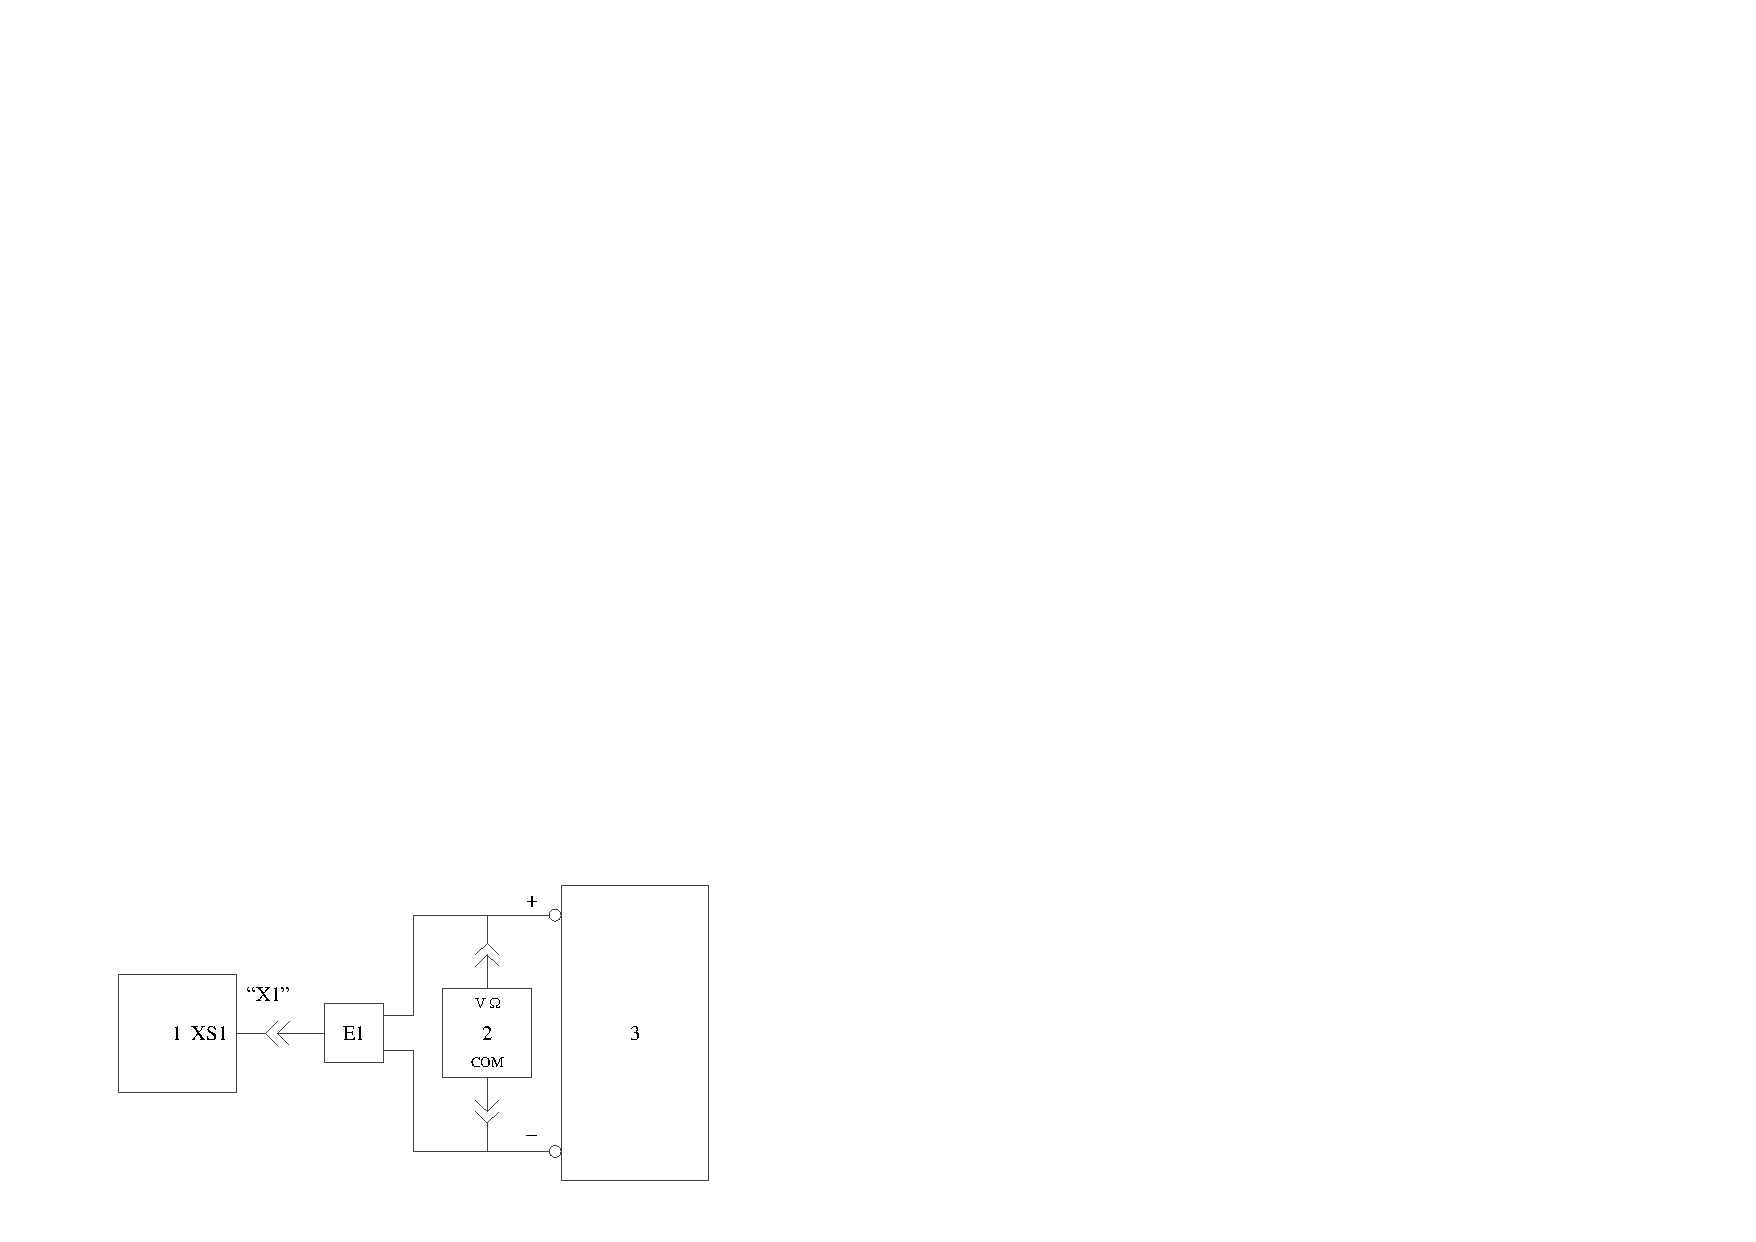
\includegraphics[page=1]{schema}
			\begin{picdescription}
				\item \ESKDtheTitle \ \RN;
				\item\label{d:multimeter} \hyperref[e:multimeter]{Мультиметр \multimeter};
				\item\label{d:stend} \hyperref[e:stend]{\stend \ \stendRN};
			\end{picdescription}
			\begin{picdescription}[label={E\arabic* ---}, ref={E\arabic*}, before={\vspace{0pt}\small}]
				\item\label{d:cable} \hyperref[e:cable]{Жгут \cableRN}.
			\end{picdescription}
			\caption{Схема проверки номинальной ёмкости, номинального напряжения, автоматической защиты от глубокого разряда в нормальных условиях}
			\label{fig:capacity}
		\end{figure}
%
	\item\label{itm:cap4} средства измерения подготавливают к работе согласно прилагаемым к ним инструкциям по эксплуатации; 
	\item\label{itm:cap5} переключают мультиметр~\ref{d:multimeter} в режим измерения сопротивления;
	\item\label{itm:cap6} измеряют сопротивление Стенда нагрузочного~\ref{d:stend} и продолжают проверку, если сопротивление составляет~$(R_{\text{н}} \pm 0,25)$~Ом, где номинальное сопротивление нагрузки~\load ;
	\item\label{itm:cap7} соединяют жгут~\ref{d:cable} со Стендом нагрузочным~\ref{d:stend};
	\item\label{itm:cap8} переключают мультиметр~\ref{d:multimeter} в режим измерения напряжения;
	\item\label{itm:cap9} измеряют исходное значение напряжения $U$ с помощью мультиметра~\ref{d:multimeter};
	\item измеряют напряжение $U_i$ каждые $\Delta t = (60 \pm 5)$~мин до снижения напряжения $U_i$ до значения ($21,0 \pm 0,5$)~В;
	\item рассчитывают ёмкость \dut \ по формуле~\eqref{eq:capacity}:
		\begin{equation}\label{eq:capacity}
			C = \sum_{i=1}^{n} \frac{U_i}{R_\text{н}},
		\end{equation}
		где $i$ "--- номер измерения, $n$ "--- количество измерений.
\end{enumerate}
 
\dut \ считают выдержавшим проверку по \ref{t_capacity} настоящих~ТУ, если рассчитанное во время испытания значение ёмкости соответствует указанному в \ref{t_capacity}.
	\point	
	\label{m_volt}
	Проверку \dut \ на соответствие \ref{t_volt} настоящих~ТУ производят следующим образом:
%
\begin{enumerate}
	\item \dut \ заряжают согласно \ref{m_charge};
	\item \dut \ выдерживают при нормальной температуре окружающей среды не менее $2$~ч;
	\item собирают схему проверки в соответствии с рисунком~\ref{fig:capacity}, не соединяя жгут~\ref{d:cable} cо Стендом нагрузочным~\ref{d:stend};
	\item средства измерения подготавливают к работе согласно прилагаемым к ним инструкциям по эксплуатации;
	\item переключают мультиметр~\ref{d:multimeter} в режим измерения сопротивления;
	\item измеряют сопротивление Стенда нагрузочного~\ref{d:stend};
	\item вычисляют отношение измеренного сопротивления нагрузки~$R$ к номинальному $R_{\text{н}}$ по формуле~\eqref{eq:load}:
		\begin{equation}\label{eq:load}
			\delta R = \frac{R}{R_{\text{н}}},
		\end{equation}
где $R_{\text{н}} = 1,25$~Ом.
	\item соединяют жгут~\ref{d:cable} со Стендом нагрузочным~\ref{d:stend};
	\item переключают мультиметр~\ref{d:multimeter} в режим измерения напряжения;
	\item измеряют напряжение $U_i$ каждые $\Delta t = (60 \pm 5)$~мин в течение~$\delta R\cdot$\work \ с помощью мультиметра~\ref{d:multimeter};
	\item вычисляют среднее значение напряжения \dut \ за время~$\delta R\cdot$\work \ по формуле~\eqref{eq:volt}:
		\begin{equation}\label{eq:volt}
			\overline U = \sum_{i=1}^{n} \frac{U_i}{n},
		\end{equation}
\end{enumerate}

Примечание "--- Допускается совмещать проверку с \ref{m_capacity}.

\dut \ считают выдержавшим проверку по \ref{t_volt} настоящих~ТУ, если рассчитанное во время испытания среднее значение напряжения \dut \ $\overline U$ не ниже номинального, указанного в \ref{t_volt}.
	\point	
	\label{m_undervolt}
	Проверку \dut \ на соответствие \ref{t_undervolt} настоящих~ТУ производят следующим образом:
%
\begin{enumerate}
	\item производят действия в соответствии с \ref{m_capacity} \ref{itm:cap1})--\ref{m_capacity} \ref{itm:cap7});
	\item контролируют значения напряжения \dut \ $U(t)$ при разряде и фиксируют значение напряжение $U_\text{мин}$, при котором выполняются условия~\eqref{eq:undervolt}:
		\begin{equation}\label{eq:undervolt}
			U(t) = \left\{\begin{array}{rl}
							U(t), & U(t) \geqslant U_\text{мин},\\
							0, & U(t) < U_\text{мин}.
						\end{array}
				\right.
		\end{equation}
\end{enumerate}

\dut \ считают выдержавшим проверку по \ref{t_undervolt} настоящих~ТУ, если зафиксированное во время испытания значение напряжения $U_\text{мин}$ не ниже значения напряжения глубокого разряда, указанного в \ref{t_undervolt}, и условие $U = 0$~В сохраняется в течение не менее~$1$~ч.
	\point	
	\label{m_short}
	Проверку \dut \ на соответствие \ref{t_short} настоящих~ТУ производят следующим образом:
%
\begin{enumerate}
	\item производят проверки \dut \ на соответствие \treb \ настоящих~ТУ;
	\item замыкают контакты жгута~\ref{d:cable} со стороны Стенда нагрузочного~\ref{d:stend}.
	\item размыкают контакты жгута~\ref{d:cable}.
	\item\label{itm:short} повторно производят проверки \dut \ на соответствие \treb \ настоящих~ТУ.
\end{enumerate}
 
\dut \ считают выдержавшим проверку по \ref{t_short} настоящих~ТУ, если в результате выполнения \ref{m_short} \ref{itm:short}) настоящих~ТУ не обнаружено отклонений от требований.
	
	\subsection{Проверка на соответствие конструктивно-техническим требованиям}
	\point
	\label{m_kt_m}
	Проверку массы по~\ref{t_kt_m} настоящих~ТУ проводят путем взвешивания полностью укомплектованного изделия на весах \hyperref[e:scales]{\scales} или других, обеспечивающих необходимый диапазон и точность измерений.

Изделие считается выдержавшим испытания по \ref{t_kt_m} настоящих~ТУ, если его масса соответствует норме, указанной в~\ref{t_kt_m} настоящих~ТУ.
	\point
	\label{m_kt_pok}
	Проверку \dut \ на соответствие требованиям \ref{t_kt_pok} настоящих~ТУ производят внешним осмотром (внешний вид оценивают визуально при дневном и искусственном освещении), сличением с чертежами на данное изделие. При необходимости производится проверка, предусмотренная стандартом на данный вид покрытия.

Оценку коррозийной стойкости, защитных свойств и механической прочности покрытий производят после климатических и механических воздействий на изделие.

На металлических и неметаллических неорганических покрытиях после всех видов испытаний допускаются следующие виды изменений, если они не влияют на работоспособность и безотказность работы изделия:
%
\begin{itemize}
	\item белый налет в виде пятен на цинковых и кадмиевых покрытиях;
	\item повреждение хроматных пленок не более чем на $10$~\% от общей поверхности;
	\item темные пятна на всех матовых покрытиях, для которых допущена разнотонность;
	\item потемнение серебряных покрытий;
	\item незначительное потускнение для всех блестящих покрытий;
	\item изменение окраски на анодно"=окисных покрытиях с наполнением красителем;
	\item следы коррозии в шлицах и на кромках крепежных деталей при возможности зачистки и последующего нанесения на эти места смазки и лака на все изделия принимаемой партии;
	\item белые точки на анодно-окисных покрытиях в количестве не более $10$~шт. на $1$~$\text{м}^2$ или не более $2$~шт. на деталях, поверхность которых менее $0,1$~$\text{м}^2$ (количество допускаемых точек на поверхностях от $0,99$~до~$0,09$~$\text{м}^2$ рассчитывать по прямо пропорциональной зависимости относительно квадратного метра).
\end{itemize}

\dut \ считается выдержавшим проверку по \ref{t_kt_pok} настоящих~ТУ, если не обнаружено отклонений от требований КД.
	
	\subsection{Проверка на соответствие требованиям по стойкости к механическим воздействиям}
%	\point
%	\label{m_m_sin_1}
%	Испытание \dut \  на прочность при воздействии синусоидальной вибрации одной частоты по~\ref{t_m_sin_1} настоящих ТУ производится на вибростенде.

\dut \ жестко крепится к платформе вибростенда в положении, при котором ось OZ направлена вверх (см.~рисунок~\ref{fig:axes} Приложения~\ref{axes}).

Испытание проводят по оси OZ на частоте, лежащей в диапазоне от 20~Гц до 30~Гц, при амплитуде виброускорения $19,6$~$\text{с}/\text{м}^2~(2g)$ в течение $30$~мин.

По окончании испытания проводят внешний осмотр \trebafter \ настоящих~ТУ с целью выявления механических повреждений, ослабления креплений и нарушения покрытий. Затем проводят проверку параметров на соответствие требованиям \treb \ настоящих~ТУ.

\dut \ считается выдержавшим проверку \ref{t_m_sin_1} настоящих~ТУ, если после испытания изделие соответствует требованиям \treb, \trebafter \ настоящих~ТУ.

	\point
	\label{m_m_shsv_st}
	Испытание на устойчивость при воздействии широкополосной случайной вибрации по \ref{t_m_shsv_st} настоящих~ТУ проводят следующим образом: 
%
\begin{enumerate}
	\item \dut \ жестко крепится к платформе вибростенда в положении, при котором координатная ось OZ направлена вертикально вверх (см. рисунок~\ref{fig:axes} Приложения~\ref{axes});
	\item собирают схему в соответствии с рисунком~\ref{fig:capacity};
	\item средства измерения подготавливают к работе согласно прилагаемым к ним инструкциям по эксплуатации;
	\item производят проверки по \treb \ настоящих~ТУ;
	\item проводят испытания \dut \ во включенном состоянии в соответствии с таблицей \ref{tab:tab_shsv};
	\item во время проведения испытания в каждом из режимов вибрации, приведенных в таблице 	\ref{tab:tab_shsv}, производится проверка \dut \ на соответствие \treb \ настоящих~ТУ.
	\item испытания \dut \ проводят в течение $1$~ч для каждой из трех взаимно перпендикулярных плоскостей;
\end{enumerate}

При отсутствии стенда, позволяющего проводить испытания на воздействие широкополосной случайной вибрации, допускается проводить испытание при воздействии синусоидальной  вибрации, плавно изменяя частоту в заданном диапазоне частот в направлении от нижней частоты до верхней и обратно со скоростью не более октавы в минуту. При этом поддерживают заданную амплитуду виброускорения или виброперемещения.

\dut \ считают выдержавшим проверку по \ref{t_m_shsv_st} настоящих~ТУ, если в процессе испытания \dut \ соответствует \treb \ настоящих~ТУ и соответствует \trebafter \ настоящих~ТУ после испытания.
	\point
	\label{m_m_ydar_mng_st}
	Испытание на устойчивость при воздействии механических ударов многократного действия по \ \ref{t_m_ydar_mng_st} настоящих~ТУ проводят следующим образом:

\begin{enumerate}
	\item \dut \ жестко крепится к платформе вибростенда в положении, при котором координатная ось OZ направлена вертикально вверх (см. рисунок~\ref{fig:axes} Приложения А);
	\item собирают схему в соответствии с рисунком~\ref{fig:capacity};
	\item средства измерения подготавливают к работе согласно прилагаемым к ним инструкциям по эксплуатации;
	\item производят проверки по \treb \ настоящих~ТУ;
	\item проводят испытания по нормам, приведенным в таблице~\ref{tab:tab_ydar_1};
	\item при проведении испытания в каждой из трех взаимно перпендикулярных плоскостей производят проверки по \treb \ настоящих~ТУ.
\end{enumerate}

\dut \ считают выдержавшим проверку по \ref{t_m_ydar_mng_st} настоящих~ТУ, если в процессе испытания он соответствует \treb \ настоящих~ТУ и \trebafter \ настоящих~ТУ после испытания.

	\point
	\label{m_m_ydar_mng_pr}
	Испытание на прочность при воздействии механических ударов многократного действия по \ref{t_m_ydar_mng_pr} настоящих~ТУ проводят следующим образом:

\begin{enumerate}
	\item \dut \ жестко крепится к платформе вибростенда в положении, при котором координатная ось OZ направлена вертикально вверх (см. рисунок~\ref{fig:axes} Приложения~\ref{axes});
	\item проводят испытания по нормам, приведенным в таблице \ref{tab:tab_ydar_2}.
\end{enumerate}

\dut \ считают выдержавшим проверку по \ref{t_m_ydar_mng_pr} настоящих~ТУ, если после испытания \dut \ соответствует \treb, \trebafter \ настоящих~ТУ.

%	\point
%	\label{m_m_transp}
%	Испытание \dut \ на прочность при транспортировании в составе объекта по \ref{t_m_transp} настоящих~ТУ проводят следующим образом:
%
\begin{enumerate}
	\item перед испытанием проводят внешний осмотр \dut \ и производят проверку по \ref{t_VSWR}, \ref{t_oslab}, \ref{t_pered}, \ref{t_isol} настоящих~ТУ;
	\item \dut \ жестко крепится к платформе вибростенда в положении, при котором ось OZ направлена вверх (см.~рисунок~\ref{fig:axes} Приложения~\ref{axes});
	\item проводят испытание по нормам таблицы \ref{tab:tab_transp} вдоль оси OZ .
\end{enumerate}

\dut \ считается выдержавшим проверку  \ref{t_m_transp} настоящих~ТУ, если после испытания изделие соответствует требованиям \ref{t_VSWR}, \ref{t_oslab}, \ref{t_pered}, \ref{t_isol}, \ref{t_kt_TY}, \ref{t_kt_pok}, \ref{t_mar_mar} настоящих~ТУ.
	\point
	\label{m_m_noise}
	Испытание \dut \ на соответствие \ref{t_m_noise}.
\subpoint
Испытание на устойчивость при воздействии акустического шума проводят в эксплуатационном положении во включенном состоянии в соответствии с ГОСТ~РВ~20.57.305 по нормам, указанным в \ref{t_m_noise}. 

Длительность испытаний должна быть не менее $15$~мин.

Перед испытанием и в процессе испытания проводят проверку \dut \ на соответствие \treb, \trebafter \ настоящих~ТУ.

\dut \ считают выдержавшим испытание, если \dut \ соответствует \treb \ настоящих~ТУ в процессе испытания и \trebafter \ настоящих~ТУ после испытания.

Примечание "--- Испытание проводят на опытных образцах и при необходимости на типовых испытаниях.

\subpoint
Испытание на прочность при воздействии акустического шума проводят в эксплуатационном положении во включенном состоянии в соответствии с ГОСТ~РВ~20.57.305 по нормам, указанным в \ref{t_m_noise}. 

Перед испытанием и в процессе испытания проводят проверку \dut \ на соответствие \treb, \trebafter \ настоящих~ТУ.

Испытание проводят во включенном состоянии. Длительность испытаний должна быть не менее $5$~ч.

По окончании испытания проверяют параметры \dut \, измеренные до начала испытаний, и производят внешний осмотр блоков с целью выявления механических повреждений, ослабления креплений.

Изделие считают выдержавшим испытание, если после испытаний оно соответствует требованиям \treb \ настоящих~ТУ и при внешнем осмотре не обнаружено механических повреждений изделия и его узлов.

Примечание "--- Испытания проводят на опытных образцах. Допускается проводить данное испытание в составе объекта.
	\point
	\label{m_m_yskor}
	Испытание на прочность и устойчивость при воздействии линейного ускорения по \ref{t_m_yskor} настоящих~ТУ проводят следующим образом:
%
\begin{enumerate}
	\item \dut \ испытывают при воздействии линейного ускорения поочередно в обоих направлениях вдоль каждой из трех взаимно перпендикулярных осей;
	\item величину  ускорения  устанавливают относительно геометрического центра \dut;
	\item погрешность значения линейного ускорения в геометрическом центре \\ должна быть не менее минус $10$~\% и не более плюс $30$~\%, при этом разница между ускорениями в геометрическом центре и в любой точке должна находиться в пределах $\pm 10$~\%; 
	\item продолжительность испытаний по каждой из трёх взаимно перпендикулярных осей должна быть не менее $3$~мин.
\end{enumerate}

\dut \ считают выдержавшим проверку по \ref{t_m_yskor} настоящих~ТУ, если после проведения испытания \treb \ соответствует \trebafter \ настоящих~ТУ.

	
	\subsection{Проверка на соответствие требованиям по стойкости к климатическим воздействиям}
	\point
	\label{m_k_p}
	Испытание на воздействие повышенной температуры среды по \ref{t_k_p} настоящих~ТУ проводят следующим образом:
%
\begin{enumerate}
	\item \dut \  помещают в камеру тепла, схему собирают в соответствии с рисунком~\ref{fig:capacity_camera};
			\begin{figure}[!htb]
			\centering
			\includegraphics[page=2]{schema}
			\begin{picdescription}
				\item \ESKDtheTitle \ \RN;
				\item \hyperref[e:multimeter]{Мультиметр \multimeter};
				\item \hyperref[e:stend]{\stend \ \stendRN};
			\end{picdescription}
			\begin{picdescription}[label={E\arabic* ---}, ref={E\arabic*}, before={\vspace{0pt}\small}]
				\item \hyperref[e:cable]{Жгут \cableRN}.
			\end{picdescription}
			\caption{Схема проверки номинальной ёмкости, номинального напряжения, автоматической защиты от глубокого разряда при воздействии климатических факторов}
			\label{fig:capacity_camera}
		\end{figure}
	\item средства измерения подготавливают к работе согласно прилагаемым к ним инструкциям по эксплуатации;
	\item производятся проверки по \treb \ настоящих~ТУ;
	\item в камере устанавливают повышенную рабочую температуру окружающей среды, указанную в~\ref{m_k_p} настоящих~ТУ; 
	\item после установления заданного значения температуры \dut \ выдерживают в камере в течение $2$~ч и производят проверки по~\treb \ настоящих~ТУ;
	\item температуру в камере повышают до повышенной рабочей кратковременной, указанной в~\ref{m_k_p} настоящих~ТУ;
	\item после прогрева \dut \ в течение $2$~ч производят проверку по \treb \ настоящих ТУ;
	\item в камере устанавливают предельную повышенную температуру окружающей среды, указанную в \ref{m_k_p} настоящих~ТУ; 
	\item после установления заданного значения температуры \dut \ выдерживают в камере в течение $6$~ч;
	\item температуру в камере понижают до повышенной рабочей;
	\item после установления заданного значения температуры \dut \ выдерживают в камере в течение $2$~ч, и производят проверки по \treb \ настоящих~ТУ;
	\item температуру  в  камере  понижают  до  нормальной  и,  после выдержки в течение $2$~ч, производят проверки по \trebafter \ настоящих~ТУ.
\end{enumerate}

\dut \  считается выдержавшим проверку по \ref{t_k_p} настоящих~ТУ, если \dut \  соответствует требованиям \treb \ настоящих~ТУ в процессе испытания и соответствует \trebafter \ настоящих~ТУ после испытания.

	\point
	\label{m_k_m}
	Испытания на воздействие пониженной температуры среды по \\ \ref{t_k_m} настоящих~ТУ проводят следующим образом:
%
\begin{enumerate}
	\item собирают схему в соответствии с рисунком \ref{fig:preheat} и прогревают \dut \ с помощью внутренней системы прогрева в течение не менее~$0,5$~ч;
	\item \dut \ помещают в камеру холода, в которой температура заранее доведена до рабочей пониженной температуры, указанной в \ref{t_k_m} настоящих~ТУ; 
	\item собирают схему проверки в соответствии с рисунком~\ref{fig:capacity_camera} в течение не более $5$ минут;
%
		\begin{figure}[!htb]
			\centering
			\includegraphics[page=4]{schema}
			\begin{picdescription}
				\item \ESKDtheTitle \ \RN;
			\end{picdescription}
			\begin{picdescription}[label={E\arabic* ---}, ref={E\arabic*}, before={\vspace{0pt}\small}]
				\item\label{d:preheat} \hyperref[e:preheat]{Жгут \preheatRN}.
			\end{picdescription}
			\caption{Схема прогрева \dut \ }
			\label{fig:preheat}
		\end{figure}
%
	\item средства измерения подготавливают к работе согласно прилагаемым к ним инструкциям по эксплуатации;
	\item производят проверки по \treb \ настоящих~ТУ;
	\item отсоединяют жгут \ref{d:cable} от Стенда нагрузочного \ref{d:stend};
	\item в камере устанавливают предельную пониженную температуру, указанную в \ref{t_k_m} настоящих~ТУ;
	\item после установления заданного значения предельной температуры  \dut \ выдерживают в камере не менее $24$~ч;
	\item температуру в камере повышают до нормальной и, после выдержки в течение $2$~ч, производят проверки по \treb, \trebafter \ настоящих~ТУ.
\end{enumerate}

\dut \ считается выдержавшим проверку по \ref{t_k_m} настоящих~ТУ, если \dut \ соответствует требованиям \treb \ настоящих~ТУ в процессе испытания и соответствует \trebafter \ настоящих~ТУ после испытания.
	\point
	\label{m_k_vlg}
	Испытание на воздействие повышенной влажности по \ref{t_k_vlg} настоящих~ТУ проводят следующим образом:
%
\begin{enumerate}
	\item \dut \ размещают в камере влажности и подключают в соответствии со схемой на рисунке~\ref{fig:capacity_camera} для проверки по \treb \ и подвергают воздействию непрерывно следующих друг за другом циклов продолжительностью по $12$~ч. Общее число циклов "--- $10$. Каждый цикл состоит из следующих этапов:
	\begin{enumerate}
		\item температуру в камере повышают до $40$~\degree C в течение $0,5$~ч; относительная влажность в этот период должна быть не менее $(95 \pm 3)$~\%; в течение периода повышения температуры на \dut \ должна иметь место конденсация влаги;
		\item в камере поддерживают температуру $(40 \pm 2)$~\degree C в течение \\ $5$---$8$~ч; относительная влажность в этот период должна быть \\ $(93 \pm 3)$~\%;
		\item температуру в камере понижают до $25$~\degree C в течение $2$---$4$~ч; в этот период относительная влажность должна быть не менее $95$~\%;
		\item в камере поддерживают температуру $25$~\degree C и относительную \\ влажность не менее $95$~\% до конца цикла;
		\end{enumerate}
	\item в последнем цикле температуру в камере понижают с $40$~\degree C до $35$~\degree C и поддерживают при относительной влажности $98$~\% в течение $2$---$4$~ч, при этом производят проверку \dut \ на соответствие требованию \treb \ настоящих~ТУ;
	\item в процессе испытаний через каждые 3 цикла в конце периода увлажнения при верхнем значении температуры рекомендуется проводить промежуточные проверки на соответствие требованию \treb \ настоящих~ТУ;
	\item \dut \ извлекают из камеры и после выдержки в нормальных условиях в течение $6$~ч, производят внешний осмотр \dut \ и проверку по \trebafter \ настоящих~ТУ.
\end{enumerate}

\dut \ считается выдержавшим проверку по \ref{t_k_vlg} настоящих~ТУ, если \dut \ соответствует требованиям \treb \ настоящих~ТУ в процессе испытания и соответствует \trebafter \ настоящих~ТУ после испытания.
	\point
	\label{m_k_ckl}
	Испытание на воздействие изменения температуры окружающей среды по \ref{t_k_ckl} настоящих~ТУ проводят следующим образом:
%
\begin{enumerate}
	\item \dut \ помещают в термокамеру;
	\item понижают температуру в камере до \kmmax \ и выдерживают при этой температуре $2$~ч;
	\item рекомендуется устанавливать скорость изменения температуры в камере при охлаждении $1$~\degree $\text{C}/\text{мин}$;
	\item температуру в камере повышают до \kpmax \ и выдерживают \dut \ при этой температуре в течение $2$~ч;
	\item скорость изменения температуры в камере при нагревании рекомендуется устанавливать не более $2$~\degree $\text{C}/\text{мин}$;
	\item после истечения времени выдержки при предельной повышенной температуре окружающей среды цикл испытания повторяют еще дважды.
\end{enumerate}

После окончания последнего цикла испытаний \dut \ извлекают из термокамеры и выдерживают в нормальных условиях $2$~ч, производят внешний осмотр и проверки по \treb, \trebafter \ настоящих~ТУ. 

\dut \  считают выдержавшим испытание, если \dut \ соответствует требованиям \treb, \trebafter \ настоящих~ТУ.
%	\point
%	\label{m_k_dav}
%	Испытание на воздействие атмосферного пониженного давления по \ref{t_k_dav} настоящих~ТУ проводят следующим образом:

\begin{enumerate}
	\item \dut \ помещают в термобарокамеру и собирают схему для проверки по \treb \ настоящих~ТУ в соответствии с рисунком~\ref{fig:capacity_camera};
	\item средства измерения подготавливают к работе согласно прилагаемым к ним инструкциям по эксплуатации;
	\item давление в камере понижают до значения, установленного в \ref{t_k_dav} настоящих~ТУ; 
	\item \dut \ выдерживают при заданном давлении в течение $1$~ч, затем производят проверку по \treb \ настоящих~ТУ;
\end{enumerate}

\dut \ считается выдержавшим проверку по \ref{t_k_dav} настоящих~ТУ, если в процессе проведения испытания он соответствует \treb \ настоящих~ТУ и после испытания \dut \ соответствует \trebafter \ настоящих~ТУ.
	\point
	\label{m_k_dav_t}
	Испытание на воздействие атмосферного пониженного давления при повышенной температуре окружающей среды и высоком токе разряда по \ref{t_k_dav_t} настоящих~ТУ проводят следующим образом:

\begin{enumerate}
	\item \dut \ помещают в термобарокамеру, температуру в которой доводят до указанного в \ref{t_k_dav_t} значения, и собирают схему для проверки по \treb \ настоящих~ТУ в соответствии с рисунком~\ref{fig:capacity_camera};
	\item средства измерения подготавливают к работе согласно прилагаемым к ним инструкциям по эксплуатации;
	\item давление в камере понижают до значения, указанного в \ref{t_k_dav_t} настоящих~ТУ;
	\item температуру в камере повышают до максимально возможного значения, но не выше \kpshort; 
	\item \dut \ выдерживают при заданном давлении в течение $1$~ч, затем производят проверку по \treb \ настоящих~ТУ при значении сопротивления Стенда нагрузочного \hyperref[e:stend]{\stendRN} $(0,65 \pm 0,05)$~Ом.
\end{enumerate}

\dut \ считается выдержавшим проверку по \ref{t_k_dav_t} настоящих~ТУ, если в процессе проведения испытания он соответствует \treb \ настоящих~ТУ при номинальном значении сопротивления Стенда нагрузочного \hyperref[e:stend]{\stendRN} \ $R_\text{н} = 0,65$~Ом и после испытания \dut \ соответствует \trebafter \ настоящих~ТУ.
	\point
	\label{m_k_mist}
	Испытание на воздействие соляного (морского) тумана по \ref{t_k_mist} настоящих~ТУ проводят для проверки коррозионной стойкости материалов и покрытий, применяемых при изготовлении \dut, следующим образом:
%
\begin{enumerate}
	\item \dut \  помещают в камеру соляного тумана, в которой  устанавливают температуру $35$~\degree C и подвергают воздействию соляного раствора;
	\item \dut \ должен быть размещен так, чтобы в процессе испытания брызги раствора из аэрозольного аппарата или пульверизатора, а также капли конденсата с потолка, стен и других частей оборудования камеры не попадали на \dut;
	\item раствор для создания тумана приготавливают из расчета ($50 \pm 3$)~г хлористого натрия (NaCl по ГОСТ~4233) на $1$~л дистиллированной воды;
	\item раствор распыляют пульверизатором, центрифугой аэрозольного аппарата или другим способом. Создаваемый туман в камере должен обладать дисперсностью $1$---$10$~мкм ($95$~\% капель) и плотностью $2$---$3$~$\text{г/м}^3$;
	\item раствор распыляют в течение $15$~мин через каждые $45$~мин.
\end{enumerate}
	
Общая продолжительность испытания "--- $2$~суток.
	
После окончания испытания \dut \ извлекают из камеры, производят внешний осмотр и проверяют на соответствие \treb, \trebafter \ настоящих~ТУ.

\dut \  считают выдержавшим проверку по \ref{t_k_mist} настоящих~ТУ, если после испытания \dut \  соответствует требованиям \treb, \trebafter \ настоящих~ТУ.

По согласованию с заказчиком допускается испытание аппаратуры заменять испытанием образцов покрытий, материалов, комплектующих изделий, коррозионная стойкость которых неизвестна.
	\point
	\label{m_k_rosa}
	%Испытания на воздействие атмосферных конденсированных осадков (инея и росы) по \ref{t_k_rosa} настоящих~ТУ проводят в следующем порядке:
%%
%\begin{enumerate}
%	\item перед испытанием производится проверка по \treb \ настоящих~ТУ;
%	\item \dut \ помещают в камеру холода и устанавливают температуру окружающей среды минус $20$~\degree C, выдерживают при этой температуре в течение $2$~ч;
%	\item \dut \ извлекают из камеры, помещают в нормальные климатические условия испытаний; 
%	\item \dut \ выдерживают в нормальных условиях в течение $3$~ч, при этом сразу после помещения \dut \ в нормальные условия и через $30$---$60$~мин производится проверка на соответствие требованиям \treb \ настоящих~ТУ.
%\end{enumerate}
Испытания на воздействие атмосферных конденсированных осадков (инея и росы) по \ref{t_k_rosa} настоящих~ТУ проводят в следующем порядке:
%
\begin{enumerate}
	\item перед испытанием производится проверка по \treb \ настоящих~ТУ;
	\item \dut \ помещают в камеру холода, устанавливают в камере температуру равную температуре точки росы и выдерживают \dut \ при этой температуре в течение $2$~ч;
	\item \dut \ извлекают из камеры, помещают в нормальные климатические условия испытаний; 
	\item \dut \ выдерживают в нормальных условиях в течение $3$~ч, при этом сразу после помещения \dut \ в нормальные условия производится проверка на соответствие требованиям \treb, \trebafter \ настоящих~ТУ.
\end{enumerate}

%Примечание "--- Допускается совмещать данное испытание с испытанием на воздействие пониженной температуры окружающей среды.

После окончания испытания производят проверку \dut \ по \trebafter \ настоящих~ТУ.

\dut \ считается выдержавшим проверку по \ref{t_k_rosa} настоящих~ТУ, если \dut \ соответствует \treb \ настоящих~ТУ в процессе испытания и соответствует \trebafter \ настоящих~ТУ после испытания.
	
	\subsection{Проверка на соответствие требованиям к материалам и комплектующим изделиям}
	\point
	\label{m_smp}
	Проверку материалов и комплектующих изделий на соответствие срокам хранения, срокам службы и ресурсов комплектующих изделий и материалов национальным или отраслевым стандартам, техническим условиям или другой НД производят по документам на их поставку, сертификатам, клеймам (другим документам, подтверждающим их приемку ОТК и \client) и документам операционного контроля в процессе производства. Проверку на входном контроле производят в соответствии с действующей на заводе-изготовителе НД.

\dut \ считается выдержавшим проверку по \ref{t_smp} настоящих~ТУ, если не обнаружено отступления от требований данного пункта.
	
%	\subsection{Проверка на соответствие требованиям к надежности}
%	\label{m_n}
%	Определение показателей надёжности на соответствие требованию \ref{t_n} настоящих~ТУ проводят методом подконтрольной эксплуатации \dut \ в составе изделия.
	
	\subsection{Проверка комплектности}
	\point
	\label{m_komp}
	Проверку по~\ref{t_komp} настоящих~ТУ производят  сравнением с комплектностью, указанной в таблице~\ref{tab:tab_komp}, оценкой правильности оформления эксплуатационной документации, состояния пломб, клейм и~т.~д. на~\dut.
%, ранее прошедших  техническую проверку ОТК и \client.

	
	\subsection{Проверка маркировки}
	\point
	\label{m_mar_ms}
	Проверку маркировки по~\ref{t_mar_ms} настоящих~ТУ  производят сличением места, содержания и способа нанесения маркировки (в том числе транспортной маркировки и маркировки упаковки) на соответствие конструкторской документации.
	
\dut \ считается выдержавшим проверку по~\ref{t_mar_ms} настоящих~ТУ, если не обнаружено отклонений от требований данного пункта.
	\point
	\label{m_mar_mar}
	Проверку качества маркировки производят визуальным осмотром состояния маркировки после окончания всех видов испытаний (механических и климатических), при этом маркировка не должна осыпаться, расплываться и выцветать.

\dut \ считается выдержавшим проверку по~\ref{t_mar_mar} настоящих~ТУ, если не обнаружено отклонений от требований данного пункта.

	
%	\subsection{Проверка требований безопасности}
%	\point
%	\label{m_kt_ps}
%	Проверку переходного сопротивления по \ref{t_kt_ps} настоящих~ТУ проводят микроомметром ИКС-5.

\dut \ считается выдержавшим испытание по \ref{t_kt_ps}, если переходное сопротивление находится в пределах, указанных в требованиях \ref{t_kt_ps} настоящих~ТУ.
	
	\subsection{Проверка консервации и упаковки}
	\label{m_up}
	\point
	\label{m_up1}
	Проверку на соответствие требованиям \ref{t_up1} (временная противокоррозийная защита) производят сравнением примененного при упаковке изделия способа защиты с требуемым вариантом защиты согласно сборочного чертежа на упаковку.

Качество противокоррозийной защиты считается удовлетворительным при положительных результатах сравнения.

	\point
	\label{m_up2}
	Проверку на соответствие требованиям \ref{t_up2} проводят сравнением способа упаковки во внутреннюю упаковку и транспортную тару, а также примененных средств для внутренней упаковки изделия с требуемым порядком упаковки, изложенным в КД на упаковку.

Качество упаковки считается удовлетворительным, если соблюдается порядок и правила упаковки, изложенные в КД.
%	\point
%	\label{m_up3}
%	Проверку на соответствие требованиям \ref{t_up3} (проверка сопроводительной документации) проводят перед пломбированием тары изделия представителем ОТК и \client, которые проверяют качество упаковки изделия, наличие комплекта монтажных частей, эксплуатационной документации, упаковочных листов, а также наличия даты консервации.

%Примечание "--- При отдельной поставке блока и при поставке изделия в составе комплекса проверку упаковки проводят по АГБП.464956.001 СБ до п.~8.

	
	\newpage
	\section{Указания по эксплуатации, в том числе требования хранения, транспортирования и утилизации изделия}
	
	\subsection{Указания по эксплуатации}
	\label{expl}	
	\point
Эксплуатация \dut \ должна осуществляться в соответствии с требованиями, изложенными в настоящих~ТУ.

\point
Перед первым использованием \dut \ следует полностью зарядить током заряда, не превышающим~$20$~А. 

\point
После неиспользования или хранения \dut \ в течение более $1$~месяца перед использованием следует повторить процедуру первичного заряда.

\point
Максимальный ток заряда и разряда "--- не более~$40$~А. 

\point
Заряжать \dut \ следует специализированным Зарядным устройством \chargerRN \ по \ref{m_charge}.	
	
	\subsection{Хранение и транспортирование}
	\label{transp}
	\point
Допускается транспортировка \dut \ всеми видами транспорта в транспортной таре изготовителя.

%\fakesubsection{}\label{transp3}
%Хранение \dut \ осуществляется в соответствии с ГОСТ~В~9.003 в условиях хранения для неотапливаемого хранилища по ГОСТ~15150.

\point
Хранение \dut \ должно осуществляться в отапливаемых помещениях при температуре воздуха от $5$ до $30$~\degree C и влажности воздуха не более $80$~\%. При этом уровень заряда (ёмкость) \dut \ по истечении $28$ суток хранения должен составлять не менее $75$~\% от начального.

\point
Допускается хранение изделия не более $1$~года в упаковке изготовителя в $(30 \pm 15)$~\% степени заряженности, в сухих отапливаемых хранилищах, складских помещениях.

\point
Запрещается хранение изделия в степени заряженности менее $5$~\%.



	\subsection{Требования утилизации изделия}
	\label{util}	
	\begin{samepage}
	\point
	\dut \ после окончания срока службы, а также признанный непригодным для практического использования, должен быть сдан в специализированные организации, имеющие право на утилизацию литий-железо-фосфатных аккумуляторов.
\end{samepage}
	
	\section{Гарантии изготовителя}
	\label{gp}
	\fakesubsection{} 
Поставщик гарантирует соответствие качества \dut \ требованиям настоящих~ТУ при соблюдении потребителем условий и правил хранения, транспортирования, монтажа и эксплуатации, установленных эксплуатационной документацией.

\fakesubsection{}
Ресурс \dut \ "--- $500$~циклов заряда"=разряда.

Срок службы \dut \ "--- $2$~года, в том числе допускается хранение изделия не более $1$~года.

%Допускается кратковременное хранение изделия (до месяца) в упаковке изготовителя в хранилищах, складских помещениях с температурой окружающего воздуха от минус $50$~\degree C до $60$~\degree C.

После $500$ циклов потеря ёмкости аккумулятора при нормальных условиях его эксплуатации не должна превышать $30$~\% от минимальной ёмкости.

\fakesubsection{}
До капитального ремонта не менее $500$~циклов заряда"=разряда.

	\ESKDappendix{Обязательное}{\normalfont Предъявительские испытания}
	\label{prav_pre}
	\fakesection{}
Предъявительские испытания готовой продукции ОТК проводит с целью контроля изделий на соответствие требованиям ТУ и определения их готовности для предъявления \client.

\fakesection{}
Предъявительские испытания проводят в объёме не менее ПСИ.

%\fakesection{}
%Каждое изделие, предъявляемое на испытание, должно быть подвергнуто в процессе изготовления технологической тренировке по инструкции \RN И5 под контролем ОТК и \client \ и производственному контролю цехом"=изготовителем на соответствие требованиям технологической документации.

\fakesection{}
На предъявительские испытания изделия предъявляют предъявительским документом, форма которого установлена изготовителем по согласованию с \client.

%\fakesection{}
%Предъявление изделий ОТК производится производственным мастером по журналу предъявления продукции ОТК, форма которого устанавливается по согласованию с ОТК.

\fakesection{}
Рабочее место и средства, используемые при контроле предъявляемых \dut, должны быть проверены, аттестованы и должны соответствовать требованиям НД и инструкции по регулировке. При невыполнении указанных требований проведение испытаний на данном рабочем месте не допускается, и извещение на испытание отклоняется с указанием конкретных причин.

\fakesection{}
Изделие считают прошедшим предъявительские испытания, если оно прошло испытания с положительным результатом, и результаты испытаний оформлены протоколом (форма~5 приложение~Д ГОСТ~РВ~15.307), а в паспорте на принятое изделие и в извещении дано заключение ОТК о годности изделия.

\fakesection{}
Изделия, принятые ОТК, должны быть опломбированы и иметь соответствующие клейма, метод простановки и расположение которых должны соответствовать комплекту документации согласно \RN.

\fakesection{}
Повторное предъявление изделия после отклонения извещения производится по устранению замечаний с актом об их устранении, подписанным мастером участка и начальником цеха или заместителем начальника цеха по технической части. Предъявление считается первичным, в извещении указывается фактическая дата предъявления изделия.

\fakesection{}
При обнаружении в изделии самоустраняющихся дефектов его возвращают изготовителю для анализа и устранения причин возникновения дефектов. Если анализ не выявляет причину отказа, то это изделие испытаниям и приемке не подлежит.

\fakesection{}
Если в результате анализа установлено, что выявленный дефект не связан с качеством изделия (неправильный режим испытаний, ошибка персонала, проводящего испытания, дефекты технологического и испытательного оборудования, проявившиеся в момент испытаний, и другие ситуации), то решение о продолжении испытания такого изделия принимает начальник ОТК после устранения причин, повлекших данный дефект.

\fakesection{}
Изделие, не выдержавшее испытание, ОТК с изложением в извещении причин забракования и возврата возвращает цеху"=изготовителю для выявления причин несоответствия изделия требованиям ТУ, проведения мероприятий по их устранению, определения возможности исправления брака (устранения или исключения дефектных изделий) и повторного предъявления. При невозможности (нецелесообразности) устранения дефектов (исключения дефектных изделий) изделие окончательно бракуют и изолируют от годных.

\fakesection{}
Возвращенное ОТК изделие после устранения дефектов (исключения дефектных изделий) и повторной проверки цехом"=изготовителем при положительных результатах допускается повторно предъявлять ОТК извещением с надписью <<Вторично>>, подписанным руководством предприятия.

К извещению должен быть приложен акт об анализе, устранении дефектов и перепроверки изделия цехом"=изготовителем и перечень проведенных мероприятий.

Форма акта устанавливается предприятием"=изготовителем.
%Форма акта устанавливается предприятием"=изготовителем и согласовывается с \client.

Если возвращенное изделие не будет повторно предъявляться, то предложение о его использовании, акт об анализе и устранении дефектов и (или) причин их возникновения цех"=изготовитель предъявляет вместе с извещением о предъявлении очередного одноименного изделия или позже в сроки, согласованные с начальником ОТК.

\fakesection{}
Повторные предъявительские испытания проводят в объеме проверок, установленных для предъявительских испытаний. В зависимости от характера дефектов, выявленных при первичных испытаниях, в отдельных технически обоснованных случаях повторные предъявительские испытания могут проводить только в объеме тех проверок, по которым выявлены несоответствия изделий установленным требованиям, которые могли повлиять на возникновение дефектов, и по которым испытания не проводились.

\fakesection{}
Окончательно забракованные по результатам предъявительских испытаний изделия изолируют от годных.

Решение об использовании окончательно забракованных изделий принимают заказчик (или по его поручению \client) и изготовитель.

\fakesection{}
Изделия, прошедшие испытания с положительными результатами, направляются на участок для полного комплектования.

\fakesection{}
Укомплектованное в соответствии с требованиями КД изделие вместе с комплектом тары для упаковки изделия начальник участка предъявляет ОТК для приемки по журналу предъявления продукции ОТК, форма которого устанавливается по согласованию с ОТК.

\fakesection{}
ОТК проводит контроль комплектности и осмотр изделия и тары по \ref{m_komp}, \ref{m_up} настоящих~ТУ. При обнаружении некомплектности изделие возвращают изготовителю, а в журнале предъявления ОТК дает заключение о причине возврата.

\fakesection{}
Изделие может быть предъявлено вновь с записью в журнале предъявления <<Вторично>> при наличии документов, подтверждающих устранение обнаруженных несоответствий и перепроверку данного комплекта изделия.

\fakesection{}
Принятые ОТК изделия предъявляются \client \ в соответствии с \ref{prav_psi} настоящих~ТУ.
	\ESKDappendix{Обязательное}{\normalfont Направления координатных осей}
	\label{axes}
	\begin{figure}[!htbp]
	\captionsetup{skip=5mm} % отступ перед подписью рисунка
	\centering
	\includegraphics[scale=0.3]{axes}
	\caption{Направления координатных осей}
	\label{fig:axes}
\end{figure}
	\ESKDappendix{Обязательное}{\normalfont Перечень средств измерений и вспомогательного оборудования, применяемых при испытаниях}
	\label{equip}
	\vspace{-1.5cm}
\begingroup
	\singlespacing
	\renewcommand{\arraystretch}{1.5}
	\small
	\centering
	\begin{longtabu} {@{}%
	|>{\setlength{\baselineskip}{0.9\baselineskip}}X[1lm]%
	|X[cm]%
	|>{\setlength{\baselineskip}{0.7\baselineskip}}X[0.55cm]%
	|X[1.3cm]%
	|X[0.25cm]%
	|>{\setlength{\baselineskip}{0.9\baselineskip}}X[1cm]|@{}}
	\captionsetup{labelformat=default}
	\caption{ }\label{tab:equip}\\
	\hline
Наименование & Тип & Класс точности, погрешность & ГОСТ, ТУ, черетж & Кол. & Завод"= изготовитель \\ \hline
	\endfirsthead
%
	\captionsetup{labelformat=continued,skip=3pt}
	\caption[]{}\\
	\hline
Наименование & Тип & Класс точности, погрешность & ГОСТ, ТУ, черетж & Кол. & Завод"= изготовитель \\ \hline
	\endhead
\multicolumn{6}{|l|}{Стандартизированные СИ:}	\\ \hline
%
	\setcounter{rowcount}{0}%
\rownumber\label{e:multimeter} \ Мультиметр &%
\multimeter & $\pm (0,06\% + 10\,\text{ед. сч.})$, $\pm (0,3\% + 30\,\text{ед. сч.})$& & 1 & APPA Technology Corp. \\ \hline
%
\rownumber\label{e:scales} \ Весы платформенные	& \scales & $50$~г	&%
ТУ~4274-029-\ 74783058-2013	& 1 &%
г.~Санкт"=Петербург ООО~<<ПетВес>>	\\ \hline
\multicolumn{6}{|l|}{Вспомогательное оборудование:} \\ \hline
	\setcounter{rowcount}{0}%
\rownumber\label{e:stend} \stend & & & \stendRN	& 1 & \company \\ \hline
\rownumber\label{e:charger} Зарядное устройство & & & \chargerRN & 1 & \company \\ \hline
\rownumber\label{e:preheat} \ Жгут & & & \preheatRN & 1 & \company \\ \hline
\rownumber\label{e:cable} \ Жгут & & & \cableRN & 1 & \company \\ \hline
\rownumber\label{e:charge} \ Жгут & & & \chargeRN & 1 & \company \\ \hline
%
\multicolumn{6}{|l|}{\parbox{175mm}{Примечания \\
	\setcounter{rowcount}{0}%
\rownumber \ Средства измерений, применяемые при испытаниях, могут быть заменены аналогичными, при этом точность заменяющих средств измерений не должна быть хуже приведенных в перечне. \\
\rownumber \ Средства измерения должны быть поверены в установленном порядке. \\
\rownumber \ Вспомогательное  оборудование  должно  проверяться в соответствии с ОСТ4Г0.005.212}} \\ \hline
	\end{longtabu}
\endgroup
	\ESKDappendix{Обязательное}{\normalfont Ссылочные нормативные документы}
	\begin{table}[H]%
	\centering
	\renewcommand{\arraystretch}{1.5}
	\caption{ }\label{tab:gost}
	\begin{tabu} {@{}|X[cm]|X[2cm]|@{}}
		\hline
Обозначение документа, на который дана ссылка & Номер раздела, подраздела, пункта, подпункта, перечисления, приложения \\ \hline
ГОСТ~РВ 20.39.304"~98 & \hyperref[1int]{Вводная часть}	\\ \hline
ГОСТ~9.014"~78	& \ref{t_up1}	\\ \hline
ГОСТ~В~25674"~83 & \ref{t_up1}	\\  \hline
ГОСТ~В~9.001"~72 & \ref{t_up2}	\\ \hline
ГОСТ~24297"~2013 & \ref{prav_op} \\ \hline
ГОСТ~РВ~15.301"~2003 & \ref{prav_op} \\ \hline
ГОСТ~РВ~15.307"~2002 & \ref{prav_pre}, \ref{prav_tip} \\ \hline
ГОСТ~РВ~20.57.305"~98	& \ref{m_m_noise}	\\ \hline
ГОСТ~4233"~77	& \ref{m_k_mist}	\\ \hline
%ГОСТ~В~9.003"~72 & \ref{transp3} \\ \hline
%ГОСТ~15150"~69 & \ref{transp3} \\ \hline
%ГОСТ~10354"~82 & \ref{m_up}	\\ \hline
%ГОСТ~3956"~76 & \ref{m_up}	\\ \hline
%ГОСТ~РВ~20.57.304"~98 & \ref{m_n_fail_1} \\ \hline
%ГОСТ~РВ~20.57.402"~81 & \ref{m_n_fail_2} \\ \hline
%ОСТ~4.091.267"~85 & \ref{m_n_fail_2} \\ \hline
ГОСТ~7328"~2001	& Приложение \ref{equip}	\\ \hline
ОСТ4.Г0.005.212 & Приложение \ref{equip}	\\ \hline
	\end{tabu}
\end{table}
	\newpage
	\begin{ESKDchangeSheet}
&	&	&	&	&	&	&	&	&	\\ \hline
&	&	&	&	&	&	&	&	&	\\ \hline
&	&	&	&	&	&	&	&	&	\\ \hline
&	&	&	&	&	&	&	&	&	\\ \hline
&	&	&	&	&	&	&	&	&	\\ \hline
&	&	&	&	&	&	&	&	&	\\ \hline
&	&	&	&	&	&	&	&	&	\\ \hline
&	&	&	&	&	&	&	&	&	\\ \hline
&	&	&	&	&	&	&	&	&	\\ \hline
&	&	&	&	&	&	&	&	&	\\ \hline
&	&	&	&	&	&	&	&	&	\\ \hline
&	&	&	&	&	&	&	&	&	\\ \hline
&	&	&	&	&	&	&	&	&	\\ \hline
&	&	&	&	&	&	&	&	&	\\ \hline
&	&	&	&	&	&	&	&	&	\\ \hline
&	&	&	&	&	&	&	&	&	\\ \hline
&	&	&	&	&	&	&	&	&	\\ \hline
&	&	&	&	&	&	&	&	&	\\ \hline
&	&	&	&	&	&	&	&	&	\\ \hline
&	&	&	&	&	&	&	&	&	\\ \hline
&	&	&	&	&	&	&	&	&	\\ \hline
&	&	&	&	&	&	&	&	&	\\ \hline
&	&	&	&	&	&	&	&	&	\\ \hline
&	&	&	&	&	&	&	&	&	\\ \hline
&	&	&	&	&	&	&	&	&	\\ \hline
&	&	&	&	&	&	&	&	&	\\ \hline
&	&	&	&	&	&	&	&	&	\\ \hline
&	&	&	&	&	&	&	&	&	\\ \hline
&	&	&	&	&	&	&	&	&	\\ \hline
\end{ESKDchangeSheet}

\end{document}
